
\chapter{Higgs $\to \tau\tau$: Results}

The extraction of the results uses a global maximum likelihood fit based on the 2D distributions in all 
channels simultaneously fit together with the control regions for the $\ttbar$, QCD multijet, and $\PW +\text{jets}$ backgrounds. 
The following section~\ref{sec:htt_2d} shows six of the tweleve distributions used in the
global maximum likelihood fit. A more detailed description of the fit and fitting process is 
laid out afterwards in section~\ref{sec:htt_fit_details}. After these two sections,
the rest of the $\htt$ results are discussed.


\section{Two-Dimensional Distributions}
\label{sec:htt_2d}
A selection of the 2D distributions used in the fit, including the three $\tauh\tauh$ distributions and
the three $\Pgm\tauh$ distributions, is shown in figures~\ref{fig:mass_tt_vbf}--\ref{fig:mass_mt_0jet}.
The choice of the binning is driven by the available statistics of the background and data templates. This leads to wider 
$\mtt$ bins and fewer slices of $\mjj$ in the poorly-populated VBF category. And, conversely, the ability of the $\Pgm\tauh$,
$\Pe\tauh$, and $\Pe\Pgm$ channels to include many slices of $\pth$ in the Boosted category. 
The most sensitive category, VBF, is shown first and is followed by the Boosted and 0-jet categories.
The signal prediction for a Higgs Boson with $\mH = 125.09\GeV$ is normalized to its best fit signal strength.
The background distributions are adjusted to the results of the global maximum likelihood fit.

\begin{figure*}[htbp]
\centering
     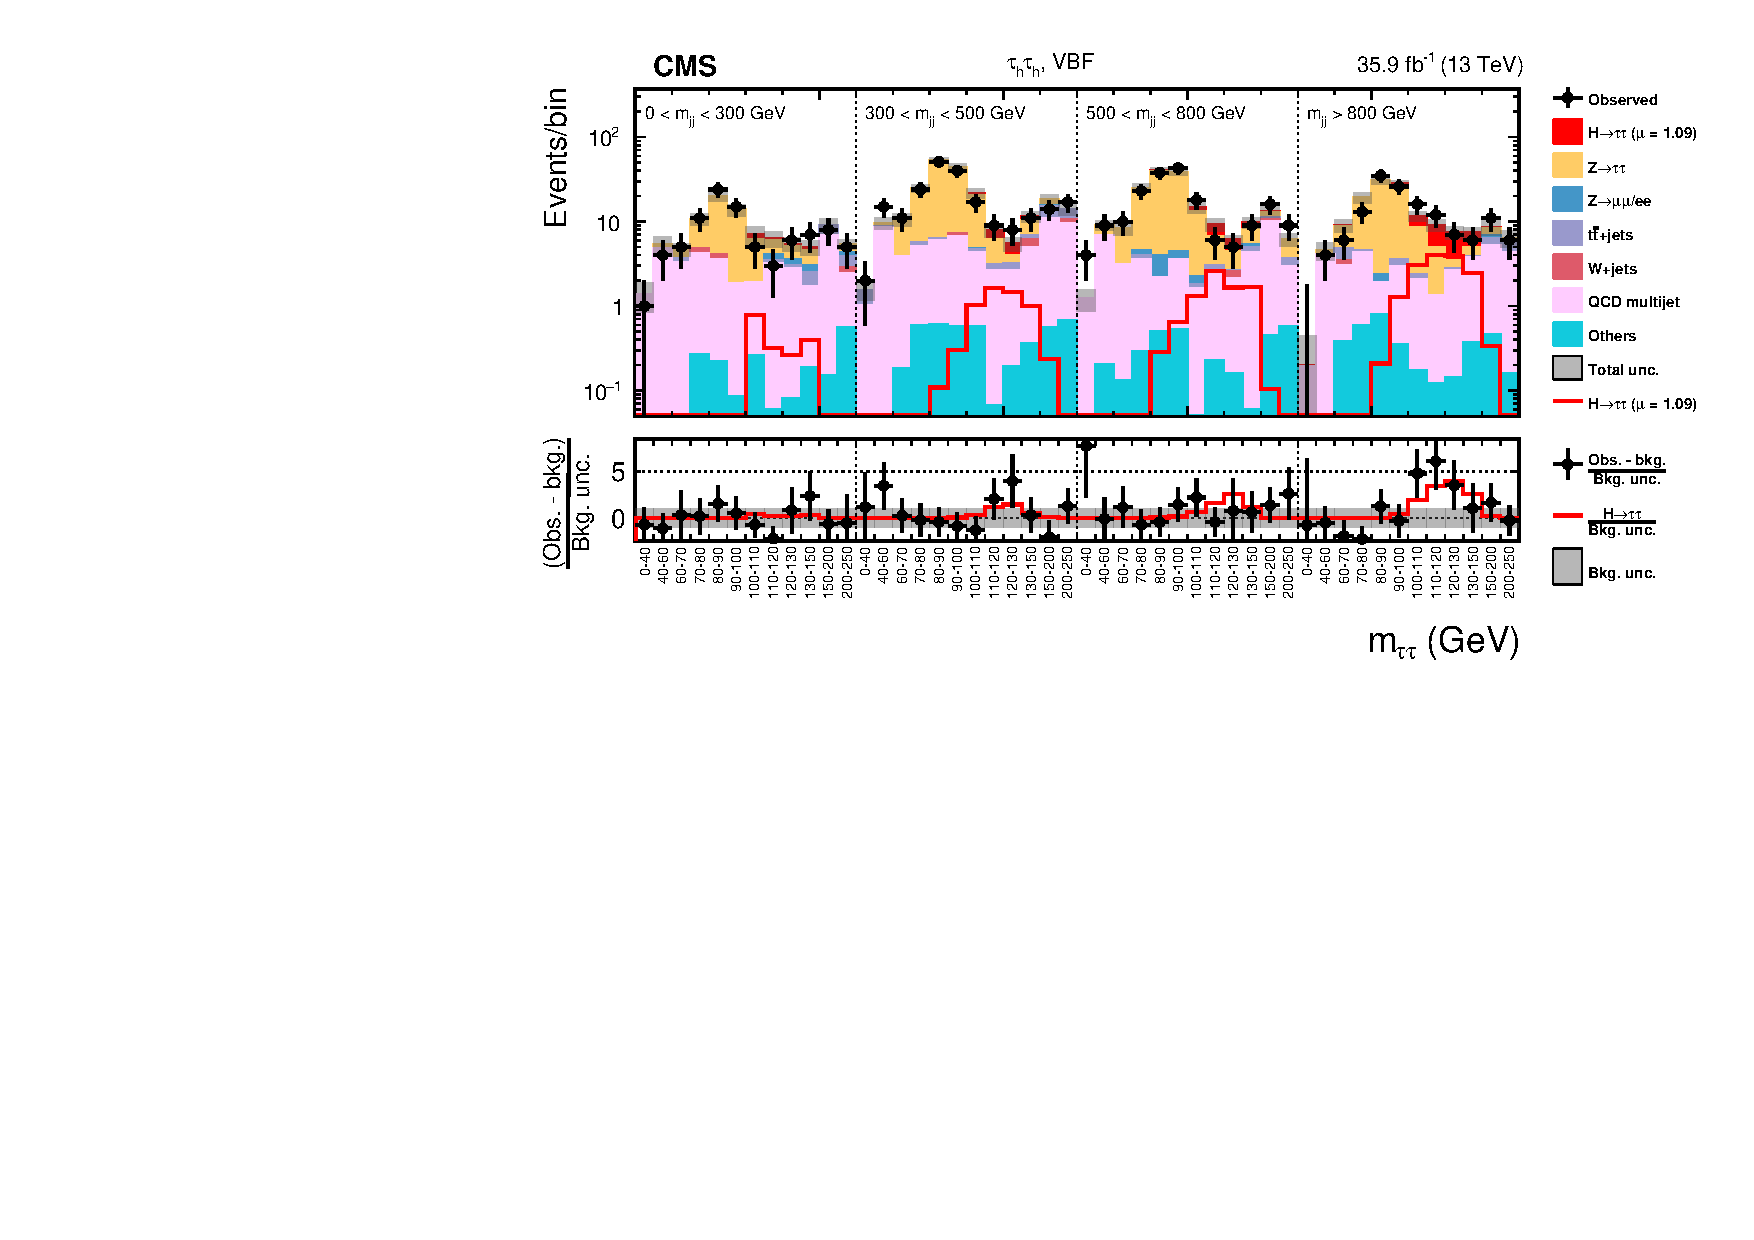
\includegraphics[width=1.0\textwidth]{higgs_to_taus/plots/Figure_006.pdf}
     \caption{
Observed and predicted 2D distributions in the VBF category of the $\tauh\tauh$ channel.
The normalization of the predicted background distributions corresponds to the result of the global fit.
The signal distribution is normalized to its best fit signal strength. The background histograms are stacked. 
The ``Others" background contribution includes events from diboson and single top quark production as well 
as Higgs Boson decays to a pair of $\PW$ bosons. The background uncertainty band accounts for all sources 
of background uncertainty, both systematic and statistical, after the global fit. 
The signal is shown both as a stacked filled histogram and as an open overlaid non-stacked histogram.
}
     \label{fig:mass_tt_vbf}
\end{figure*}

\begin{figure*}[htbp]
\centering
     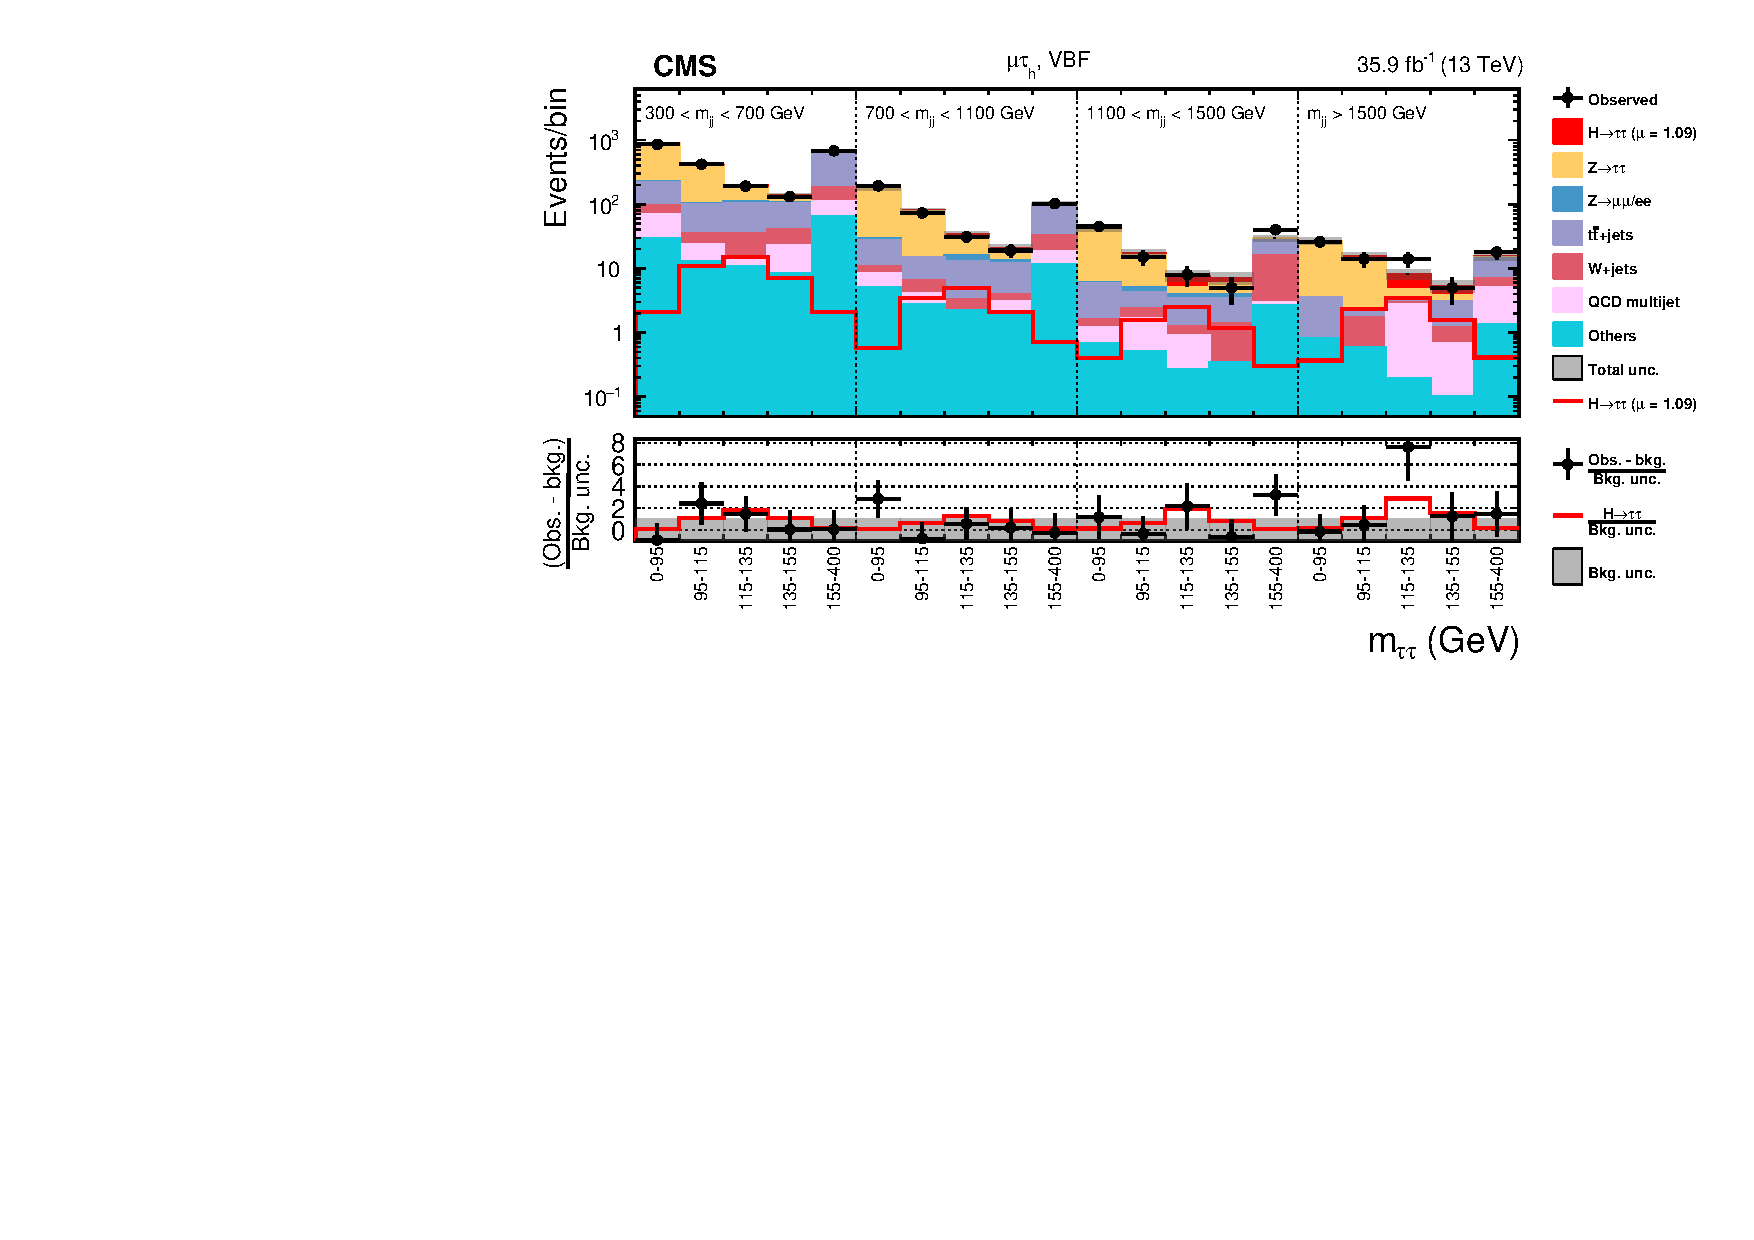
\includegraphics[width=1.0\textwidth]{higgs_to_taus/plots/Figure_007.pdf}
     \caption{Observed and predicted 2D distributions in the VBF category of the $\Pgm\tauh$ channel. The description of the histograms is the same as in figure~\ref{fig:mass_tt_vbf}.}
     \label{fig:mass_mt_vbf}
\end{figure*}

%\begin{figure*}[htbp]
%\centering
%     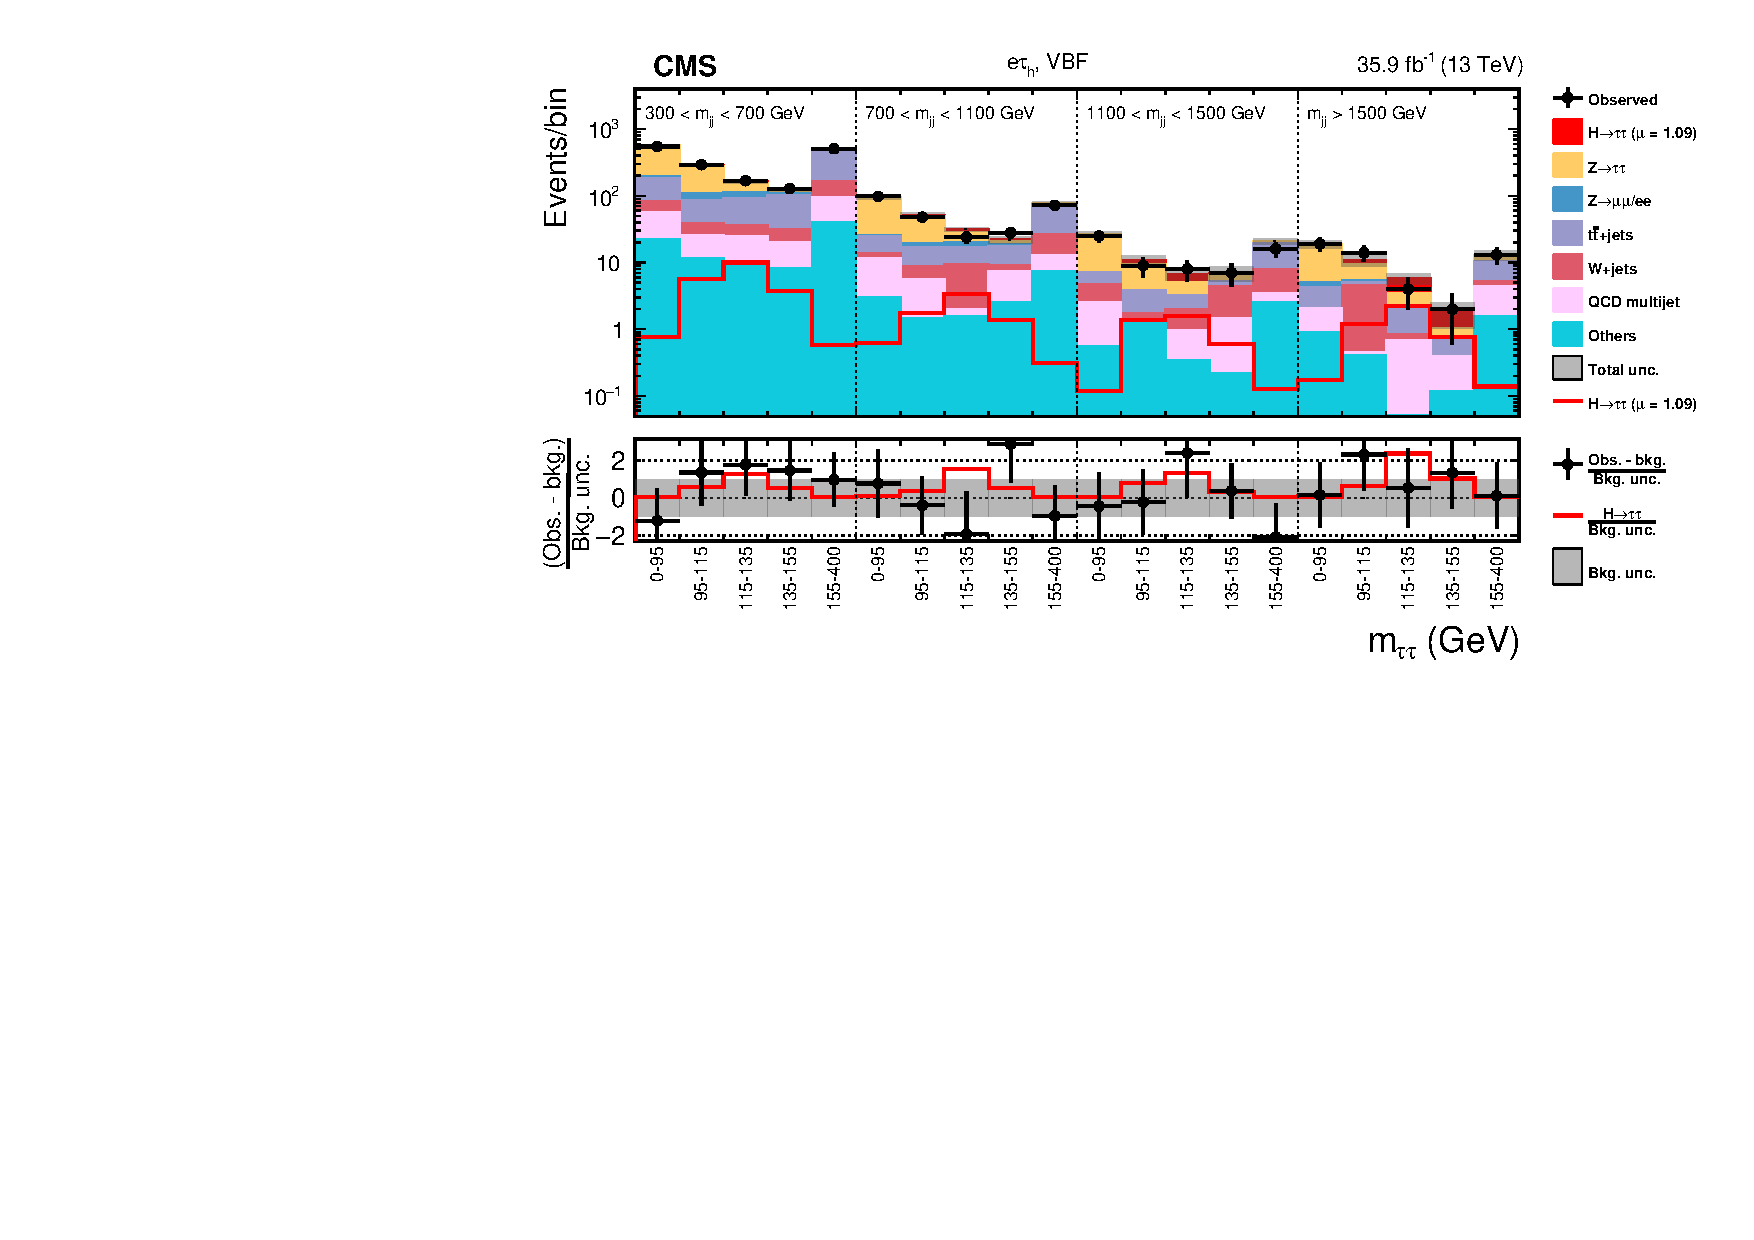
\includegraphics[width=1.0\textwidth]{higgs_to_taus/plots/Figure_008.pdf}
%     \caption{Observed and predicted 2D distributions in the VBF category of the $\Pe\tauh$ channel. The description of the histograms is the same as in figure~\ref{fig:mass_tt_vbf}.}
%     \label{fig:mass_et_vbf}
%\end{figure*}
%
%
%\begin{figure*}[htbp]
%\centering
%     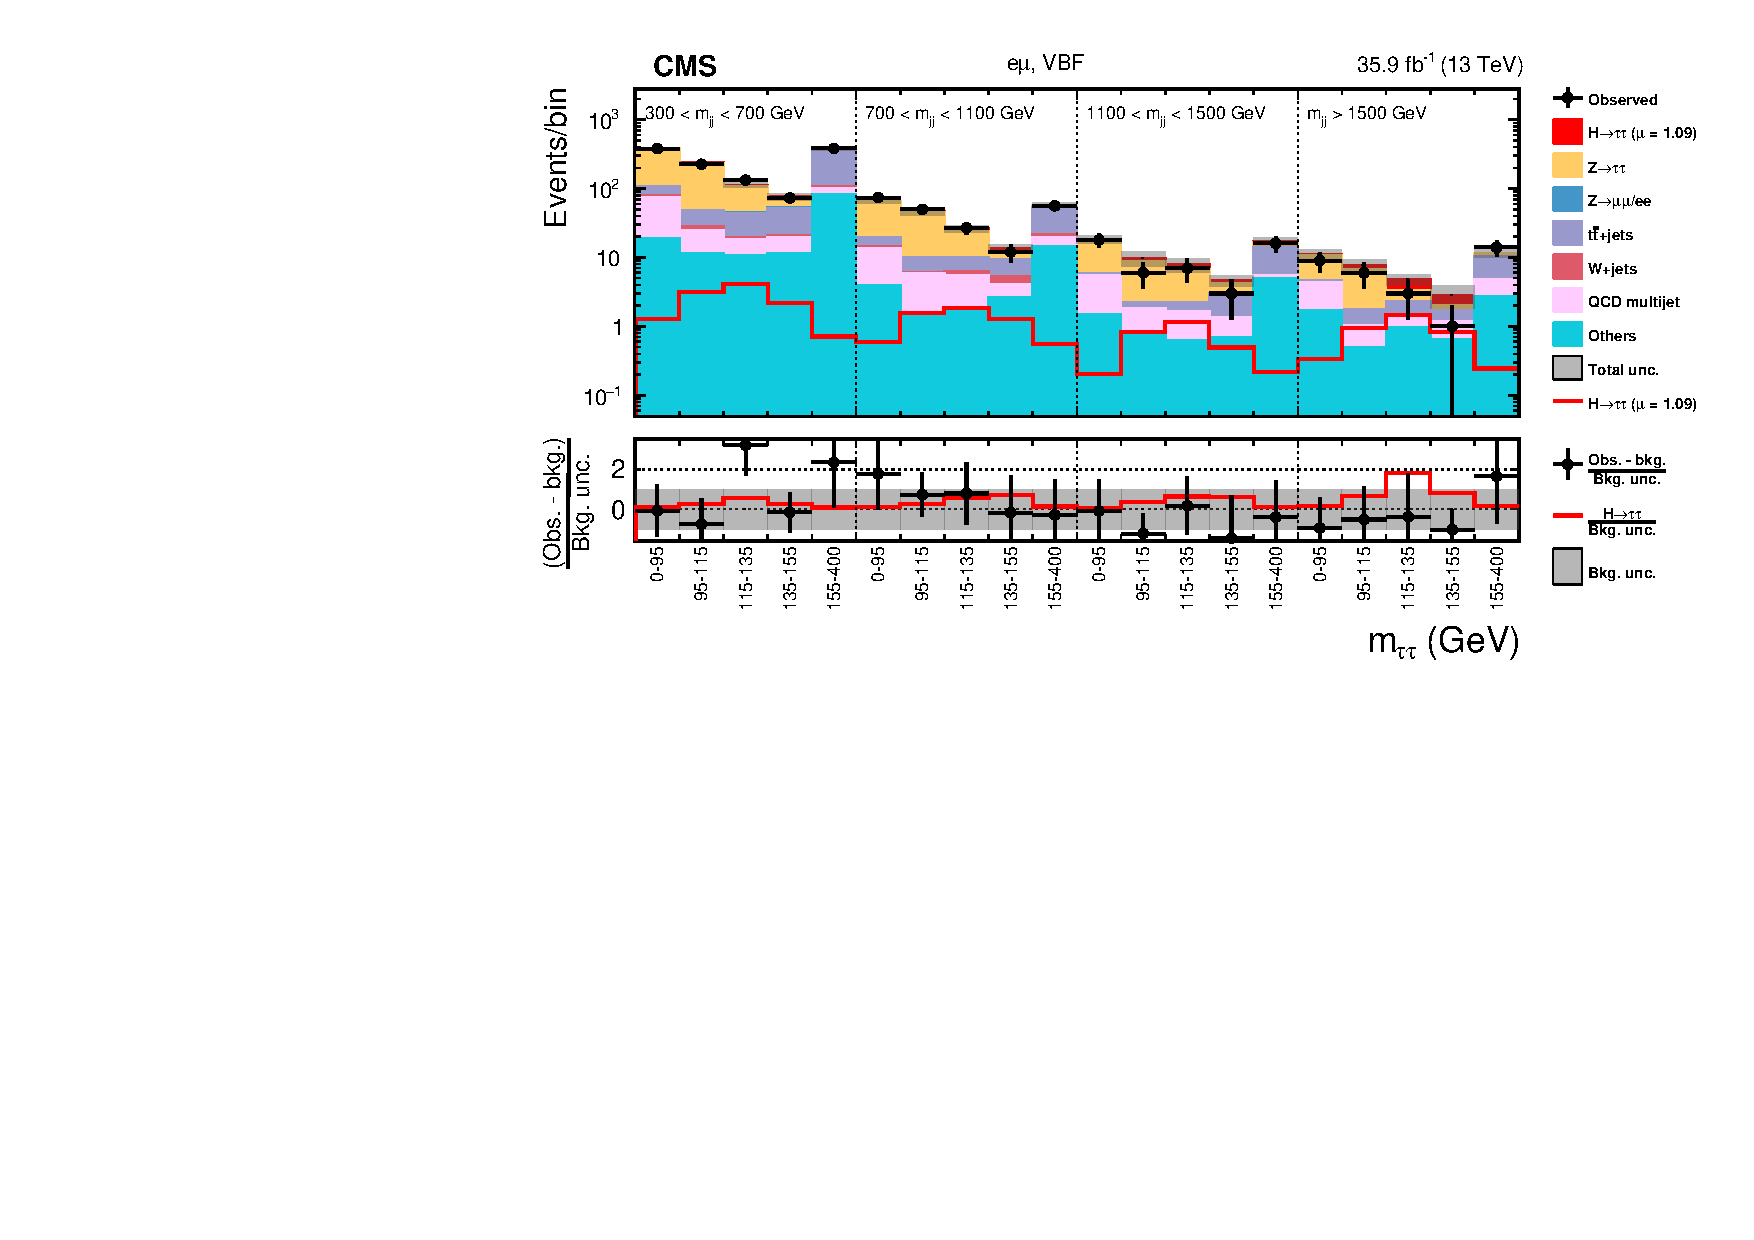
\includegraphics[width=1.0\textwidth]{higgs_to_taus/plots/Figure_009.pdf}
%     \caption{Observed and predicted 2D distributions in the VBF category of the $\Pe\Pgm$ channel. The description of the histograms is the same as in figure~\ref{fig:mass_tt_vbf}.}
%     \label{fig:mass_em_vbf}
%\end{figure*}

\begin{figure*}[htbp]
\centering
     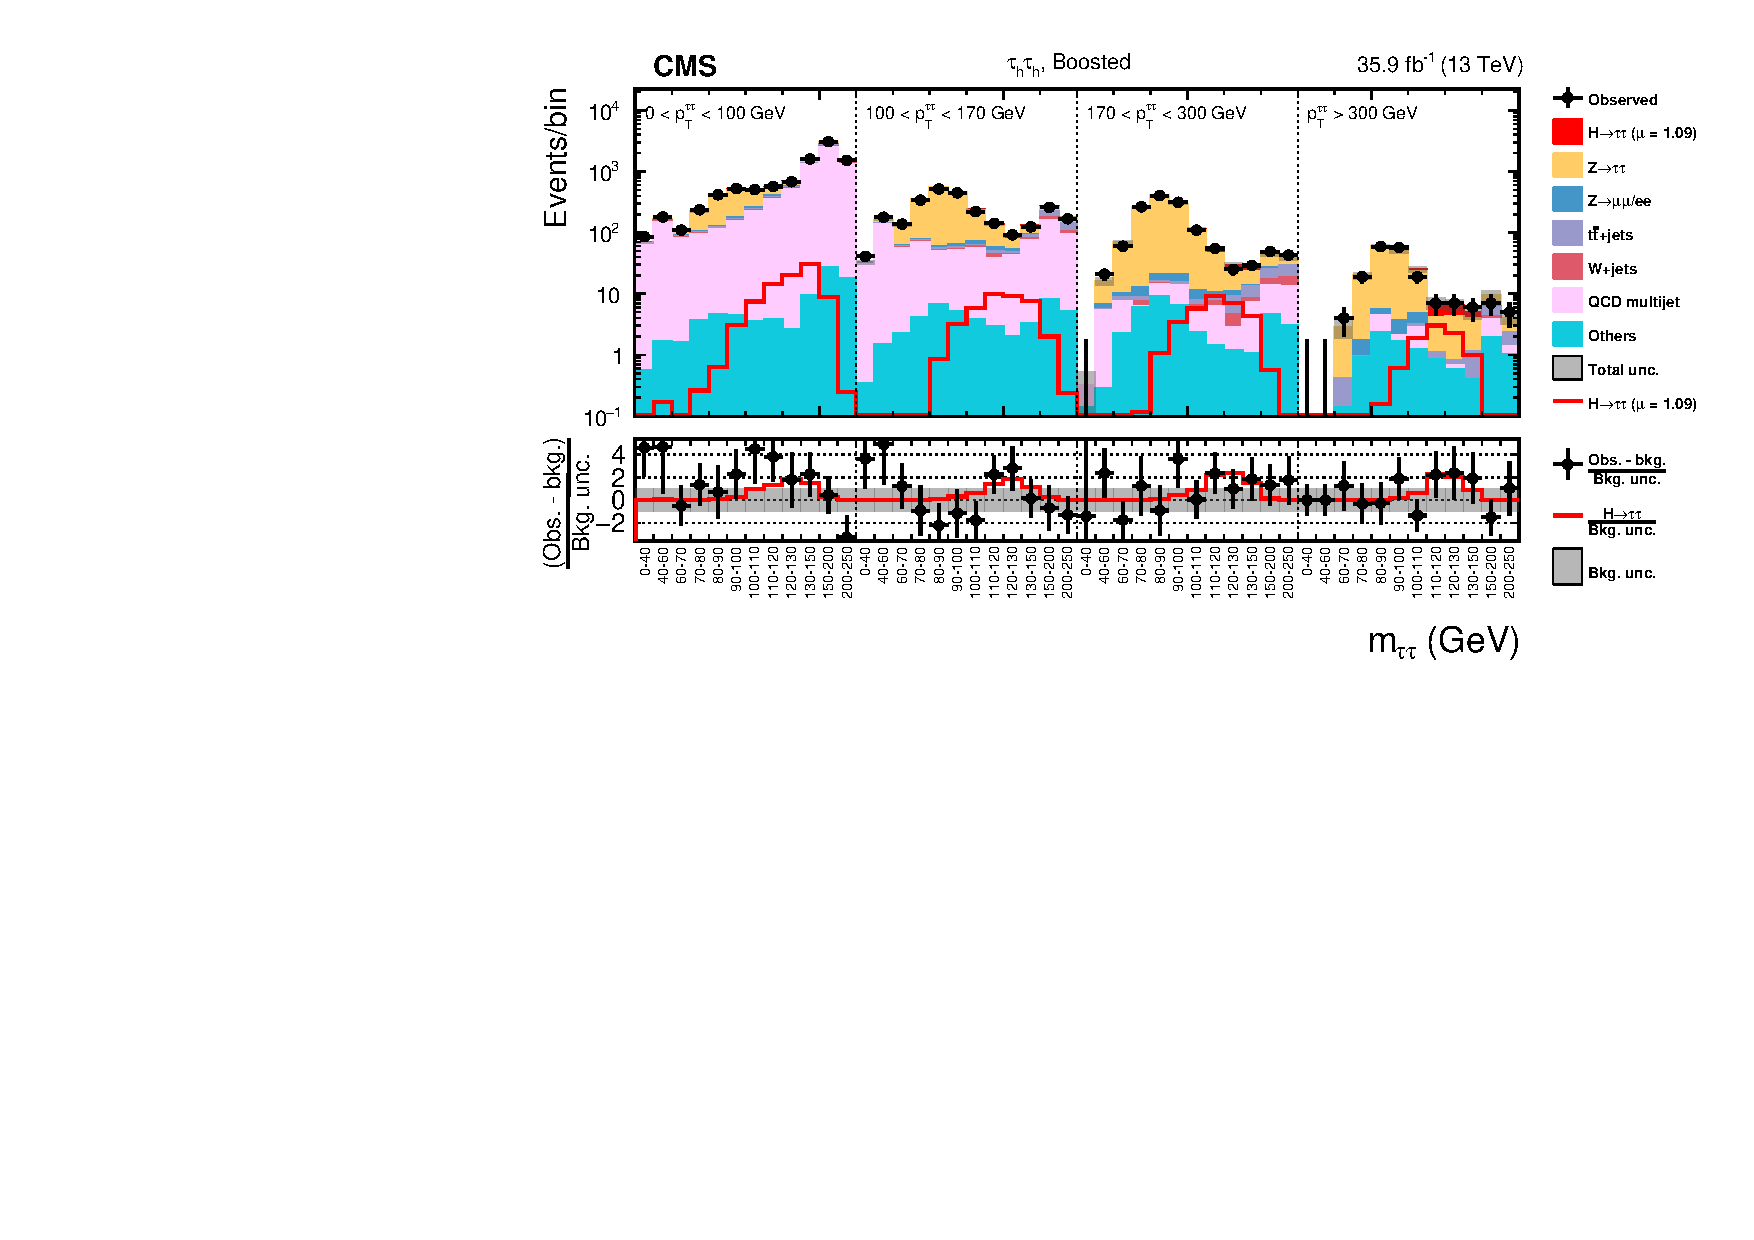
\includegraphics[width=1.0\textwidth]{higgs_to_taus/plots/Figure_010.pdf}
     \caption{Observed and predicted 2D distributions in the Boosted category of the $\tauh\tauh$ channel. The description of the histograms is the same as in figure~\ref{fig:mass_tt_vbf}.}
     \label{fig:mass_tt_boosted}
\end{figure*}

\begin{figure*}[htbp]
\centering
     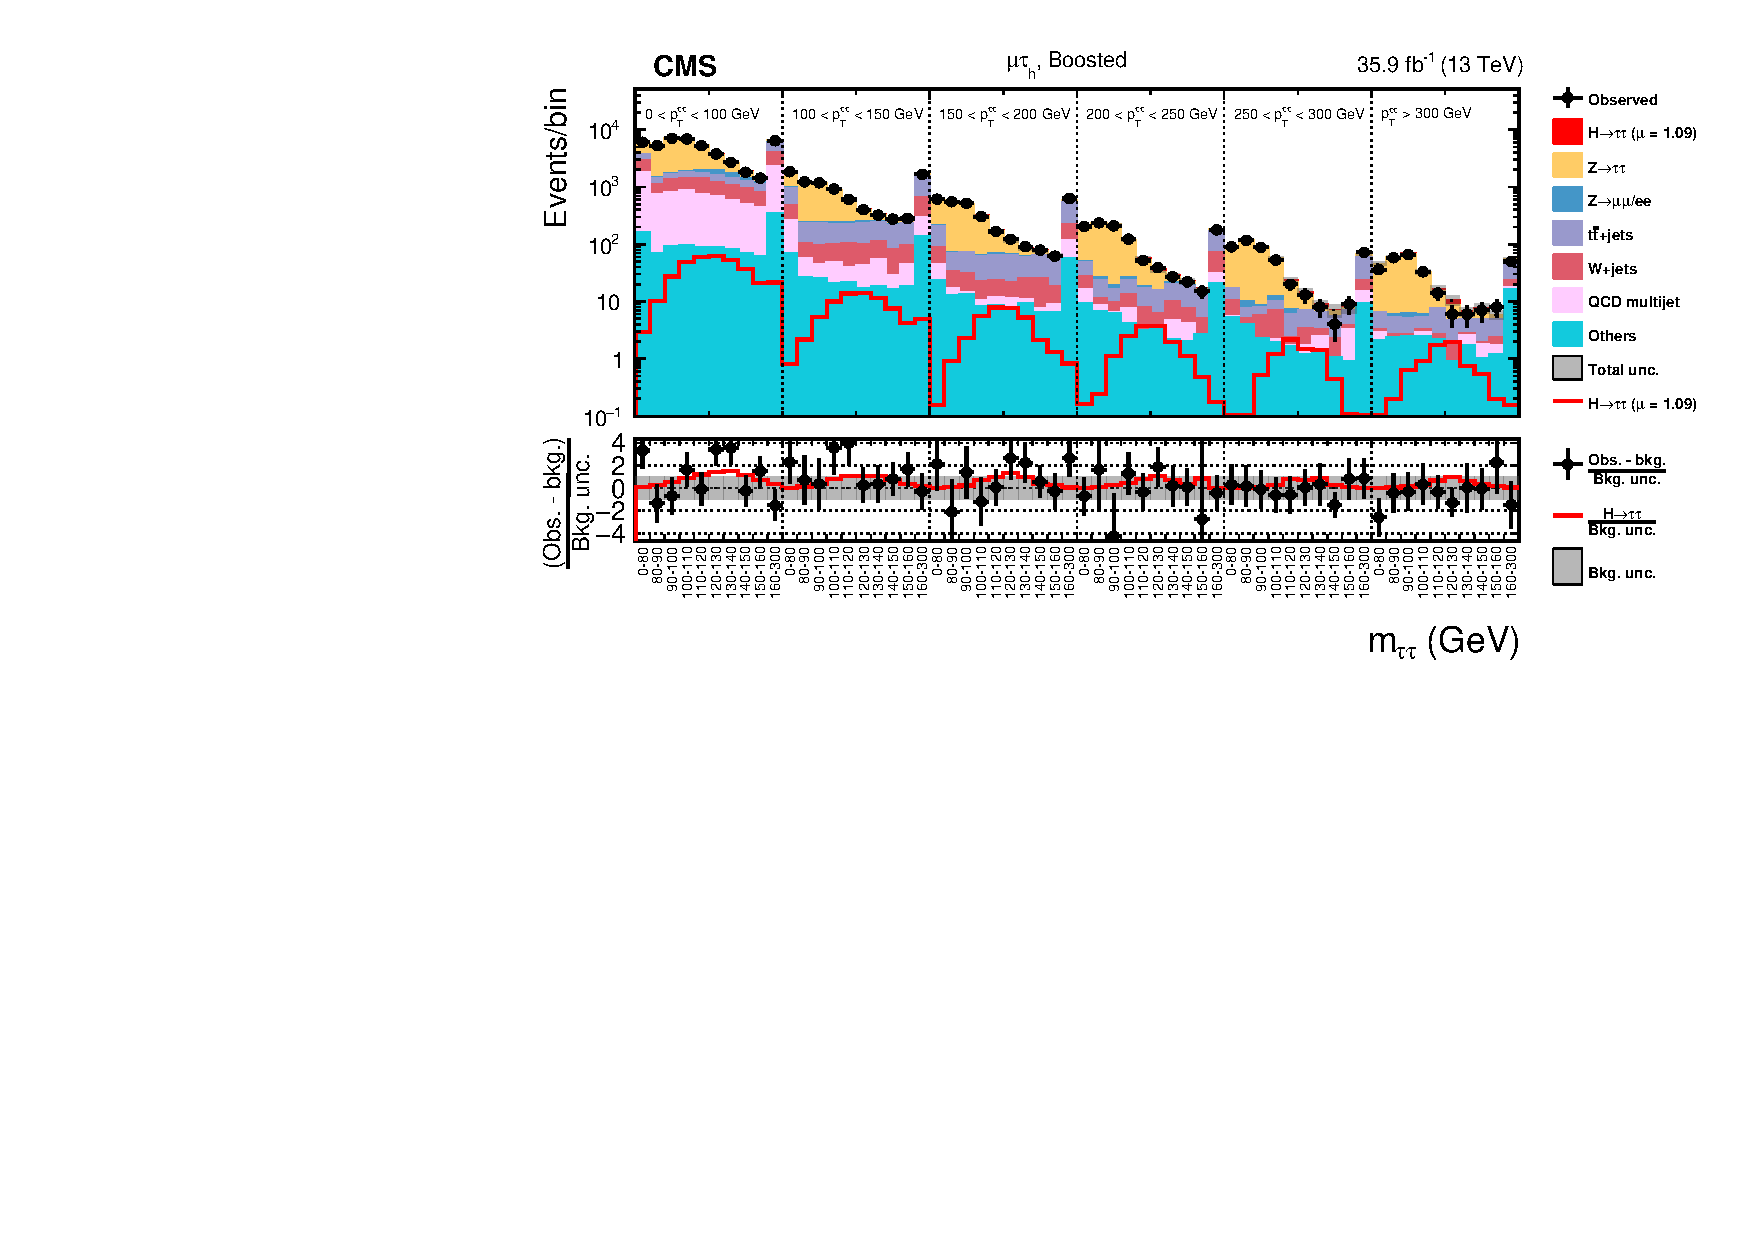
\includegraphics[width=1.0\textwidth]{higgs_to_taus/plots/Figure_011.pdf}
     \caption{Observed and predicted 2D distributions in the Boosted category of the $\Pgm\tauh$ channel. The description of the histograms is the same as in figure~\ref{fig:mass_tt_vbf}.}
     \label{fig:mass_mt_boosted}
\end{figure*}

%\begin{figure*}[htbp]
%\centering
%     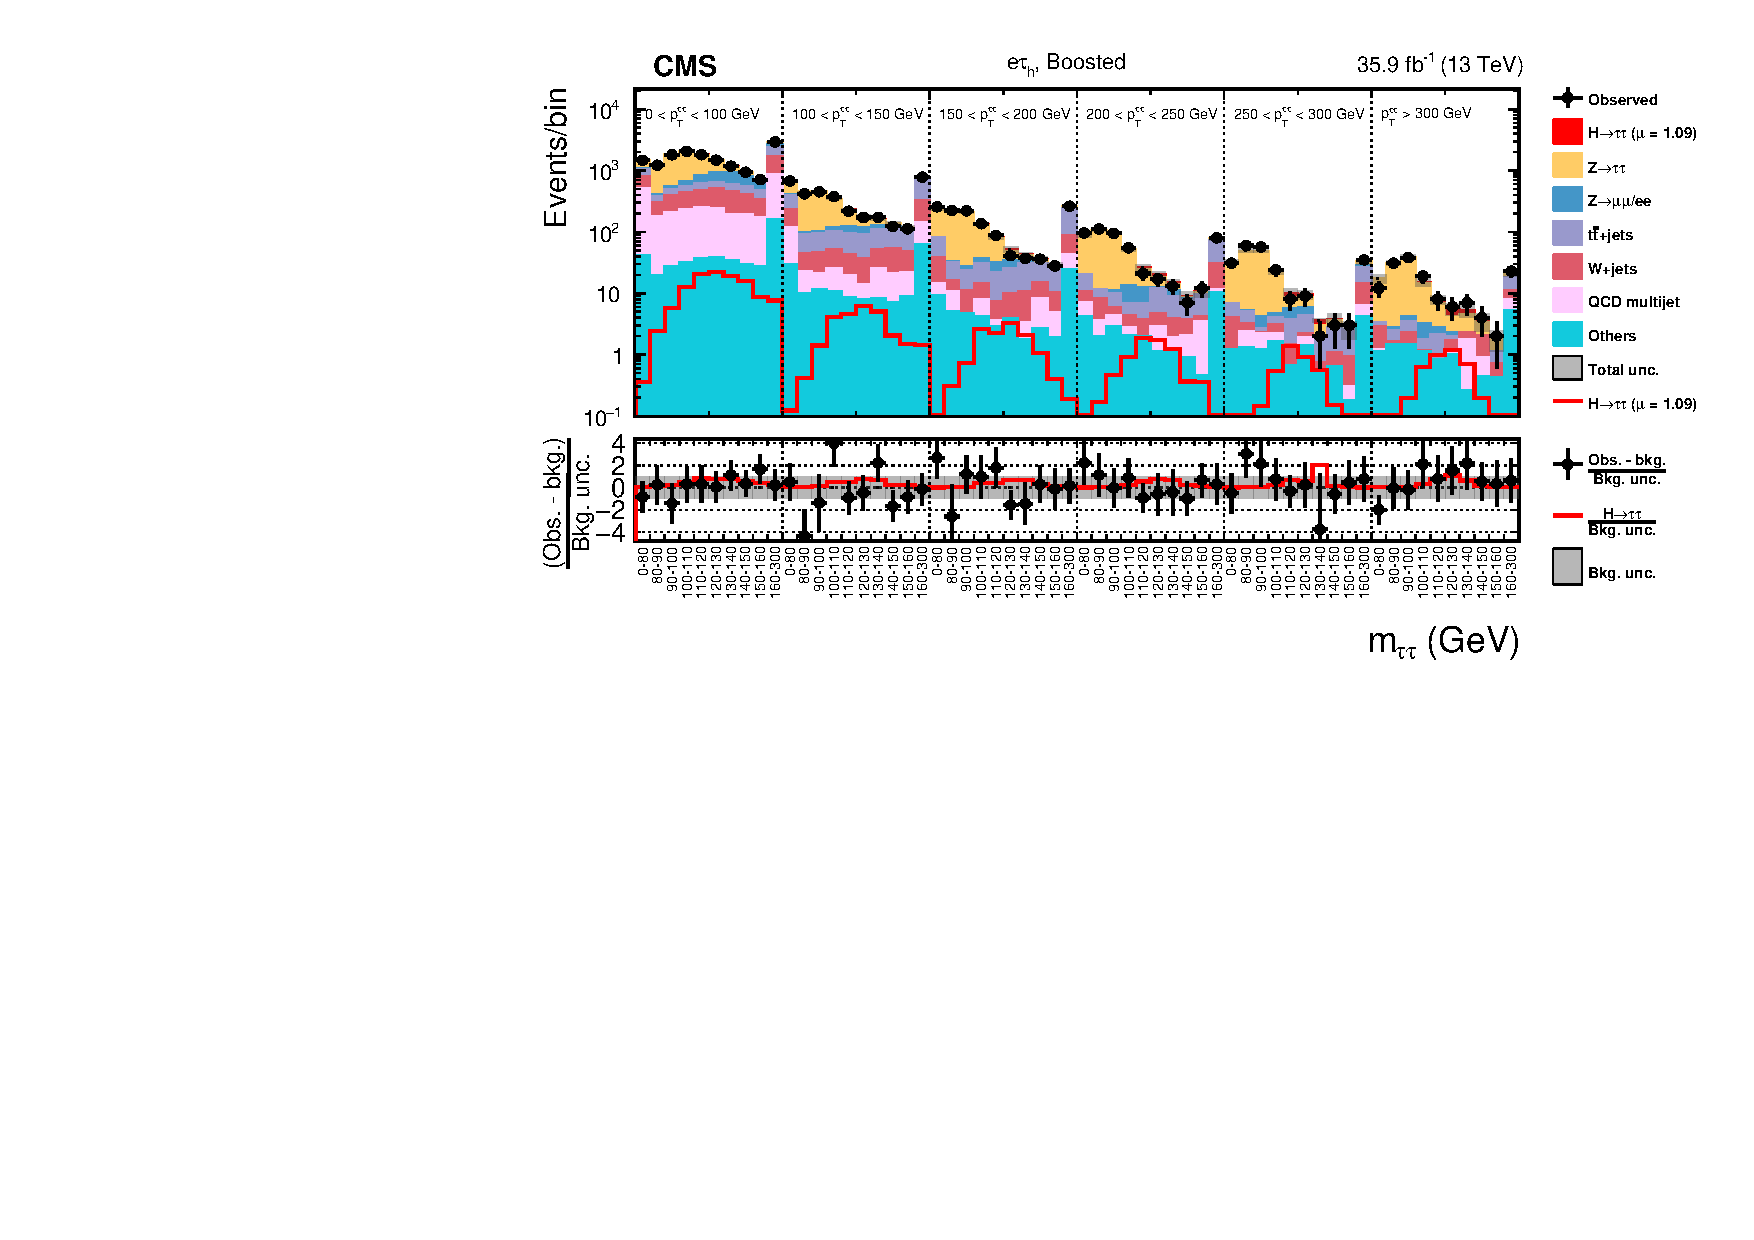
\includegraphics[width=1.0\textwidth]{higgs_to_taus/plots/Figure_012.pdf}
%     \caption{Observed and predicted 2D distributions in the Boosted category of the $\Pe\tauh$ channel. The description of the histograms is the same as in figure~\ref{fig:mass_tt_vbf}.}
%     \label{fig:mass_et_boosted}
%\end{figure*}
%
%\begin{figure*}[htbp]
%\centering
%     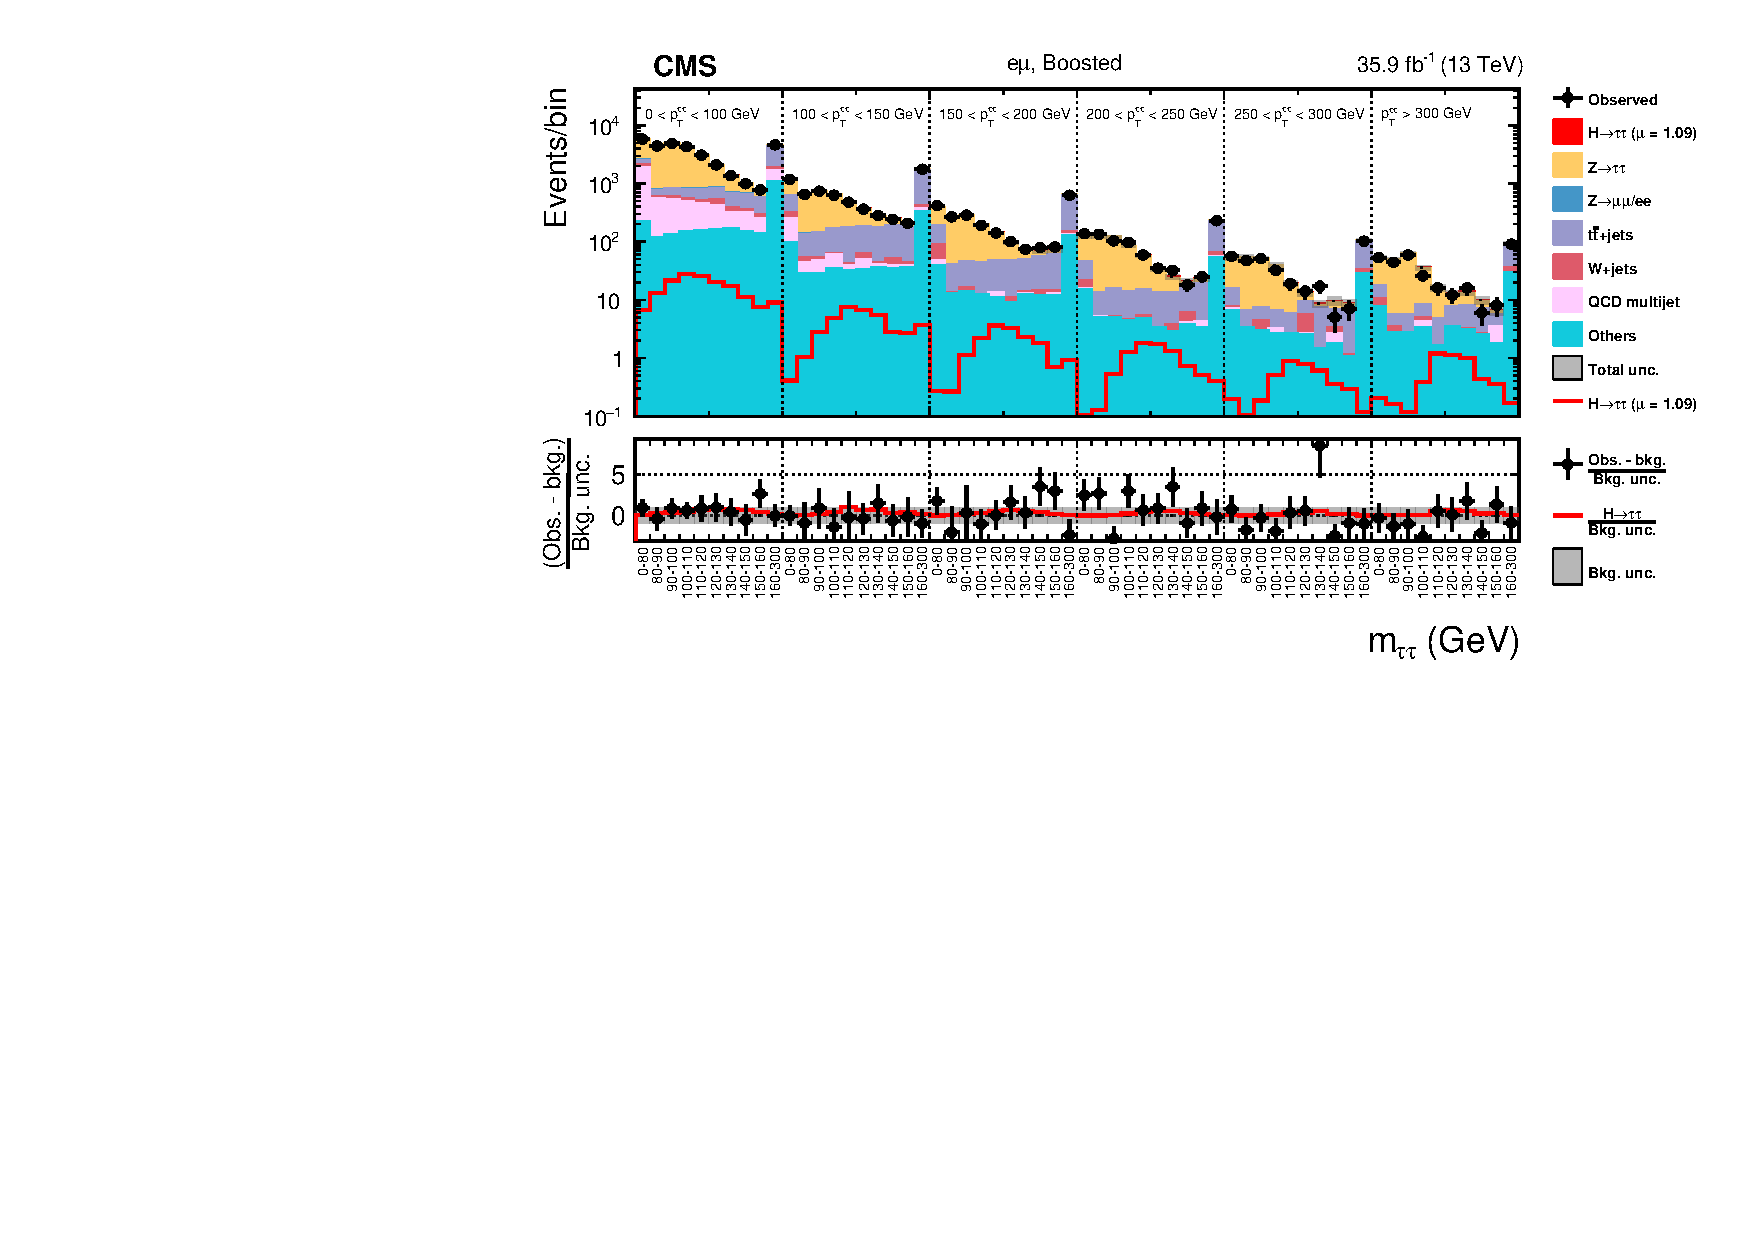
\includegraphics[width=1.0\textwidth]{higgs_to_taus/plots/Figure_013.pdf}
%     \caption{Observed and predicted 2D distributions in the Boosted category of the $\Pe\Pgm$ channel. The description of the histograms is the same as in figure~\ref{fig:mass_tt_vbf}.}
%     \label{fig:mass_em_boosted}
%\end{figure*}

\begin{figure*}[htbp]
\centering
     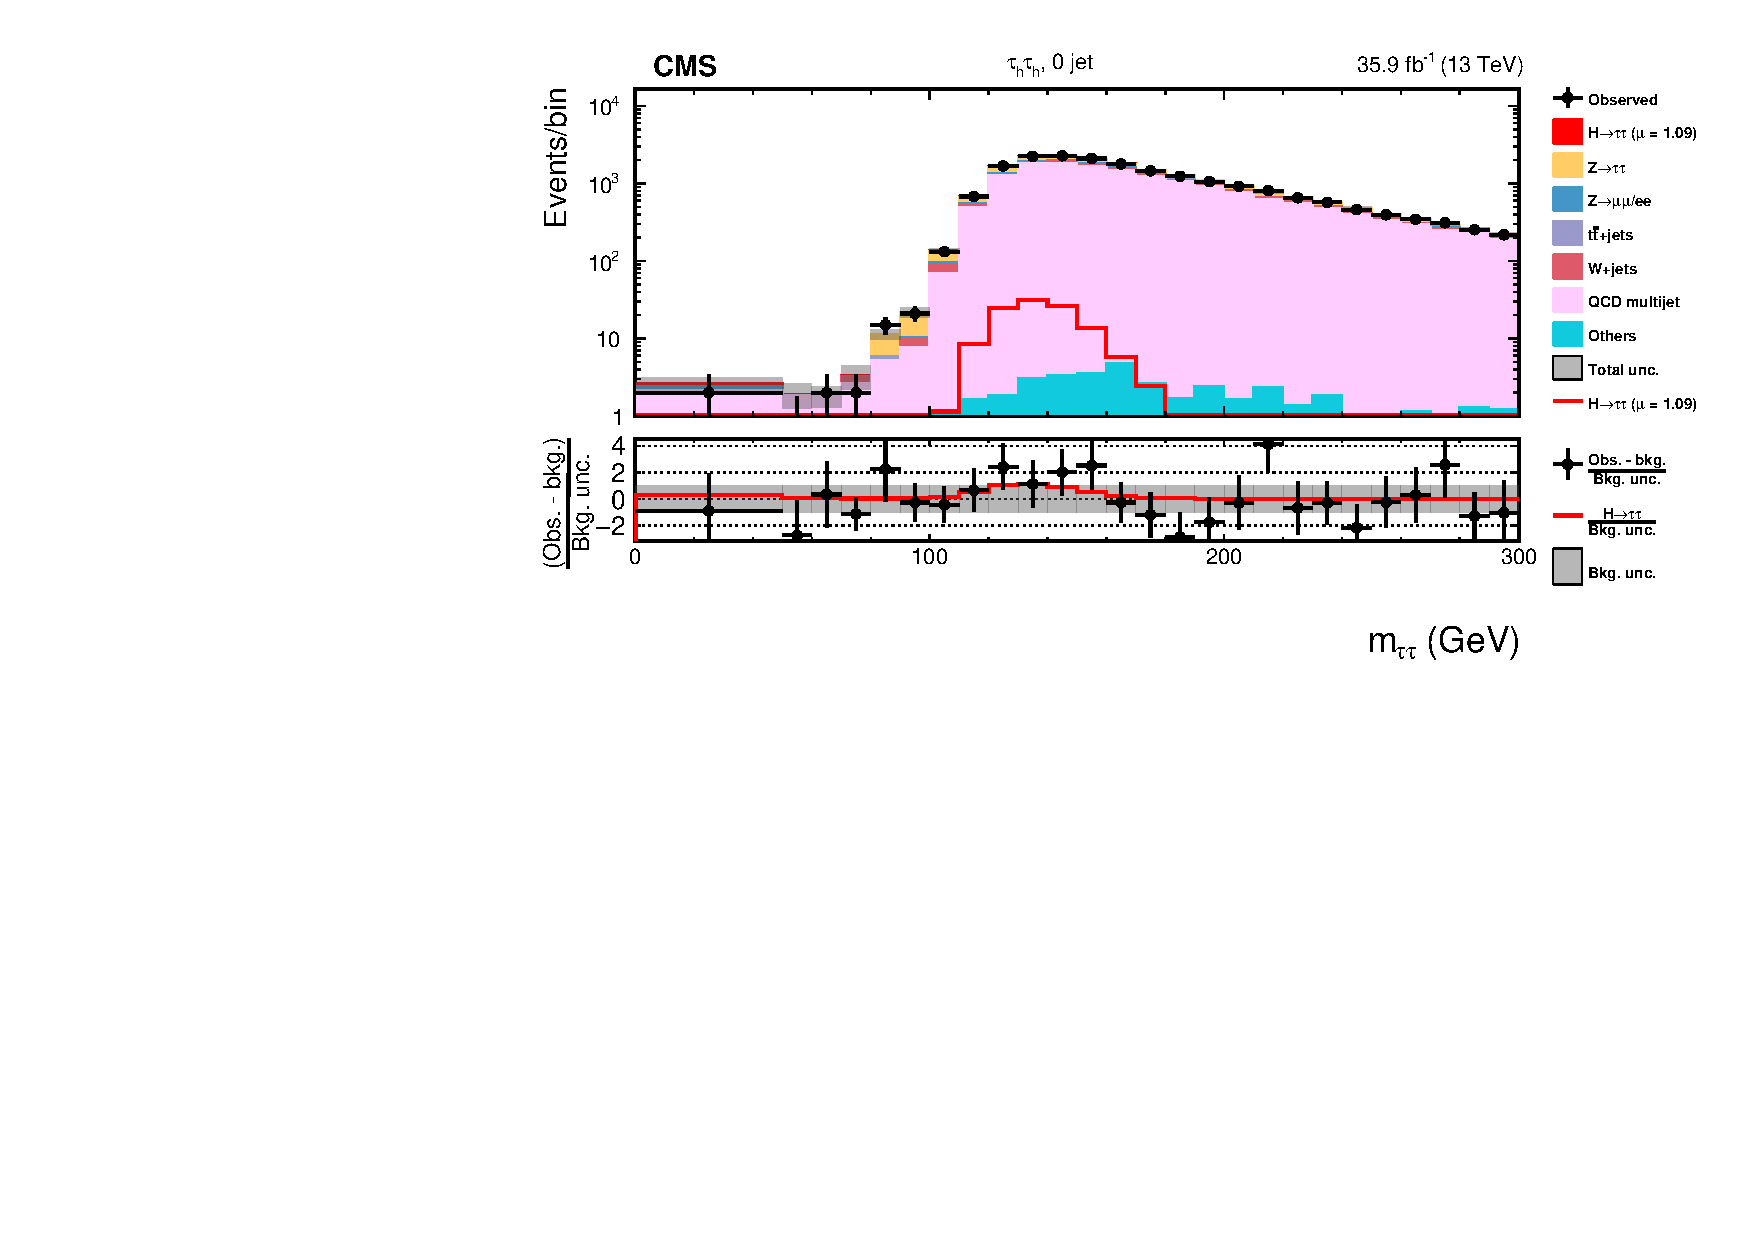
\includegraphics[width=1.0\textwidth]{higgs_to_taus/plots/Figure_014.pdf}
     \caption{Observed and predicted distributions in the 0-jet category of the $\tauh\tauh$ channel. The description of the histograms is the same as in figure~\ref{fig:mass_tt_vbf}.}
     \label{fig:mass_tt_0jet}
\end{figure*}



\begin{figure*}[htbp]
\centering
     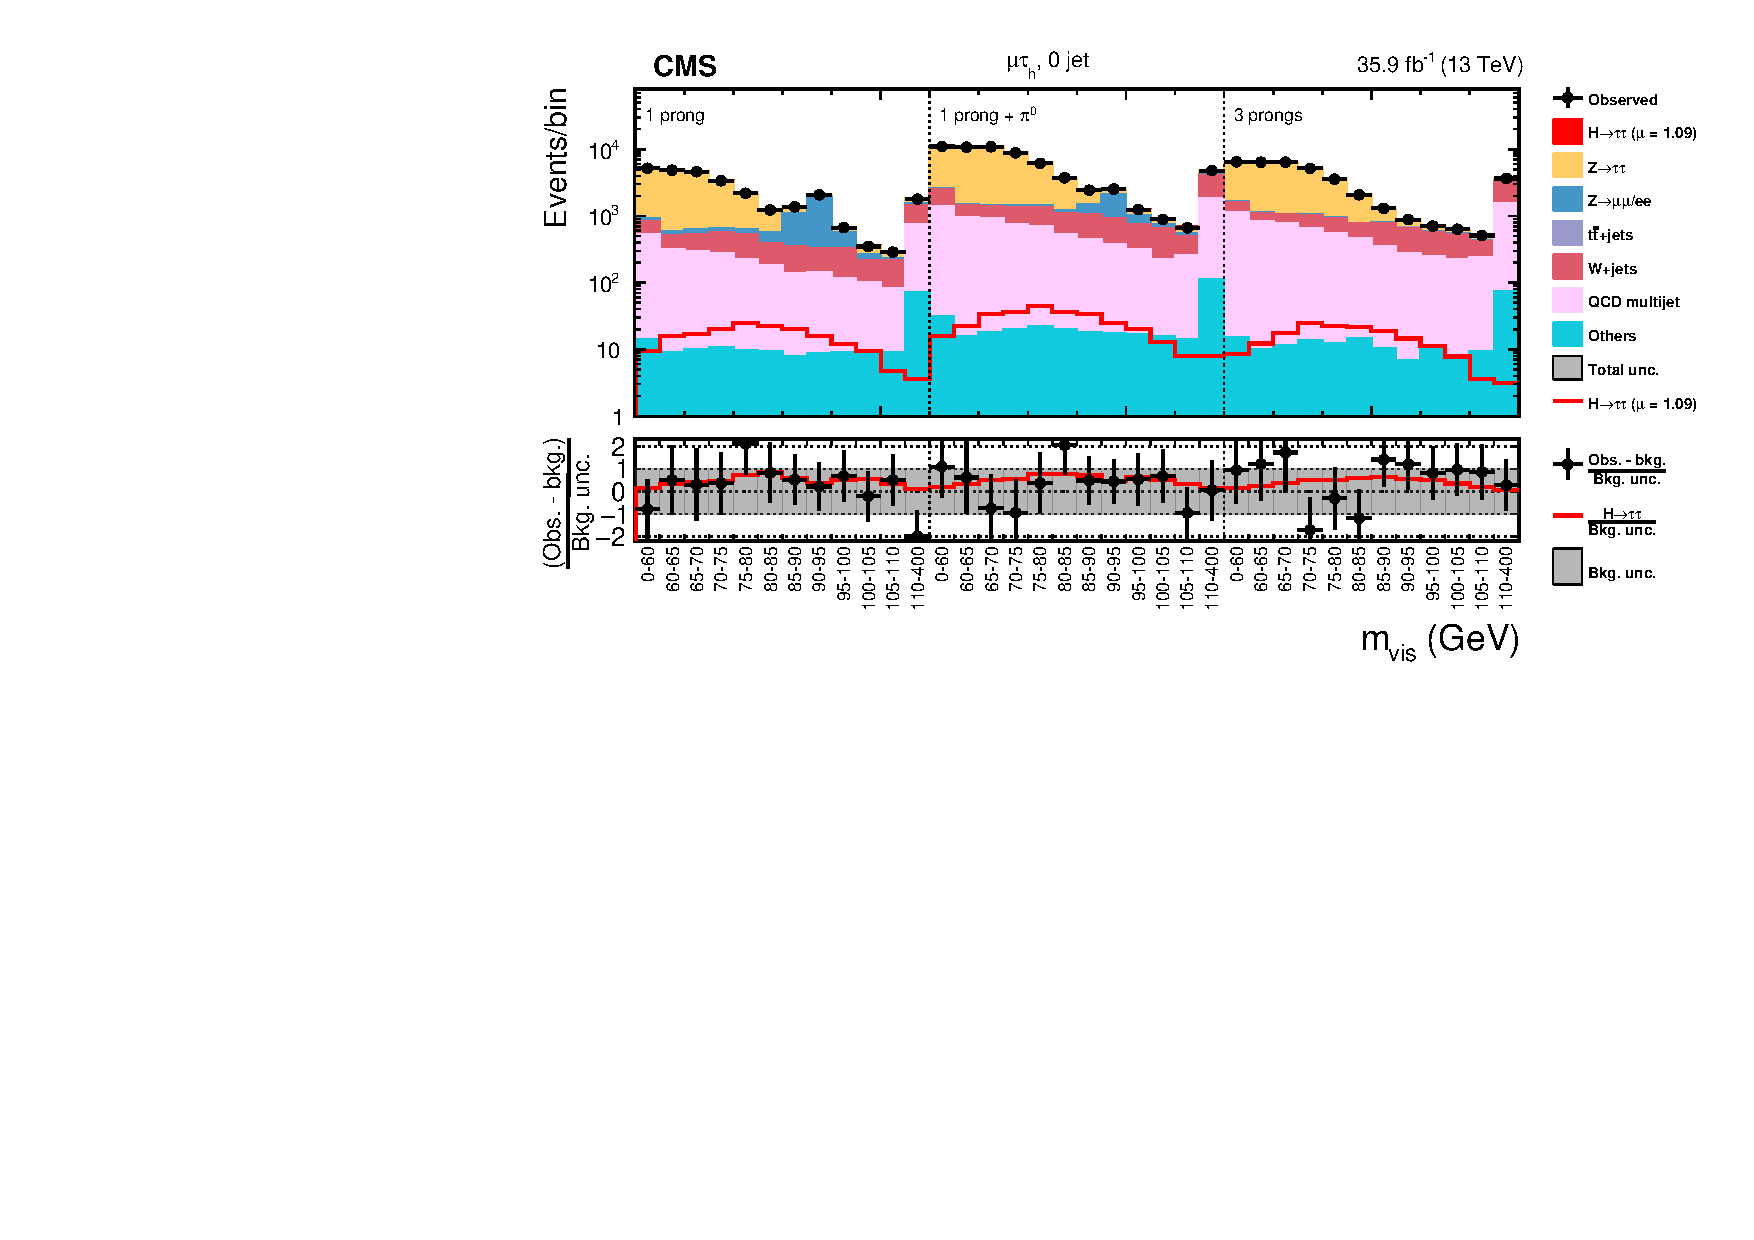
\includegraphics[width=1.0\textwidth]{higgs_to_taus/plots/Figure_015.pdf}
     \caption{Observed and predicted 2D distributions in the 0-jet category of the $\Pgm\tauh$ channel. The description of the histograms is the same as in figure~\ref{fig:mass_tt_vbf}.}
     \label{fig:mass_mt_0jet}
\end{figure*}

%\begin{figure*}[htbp]
%\centering
%     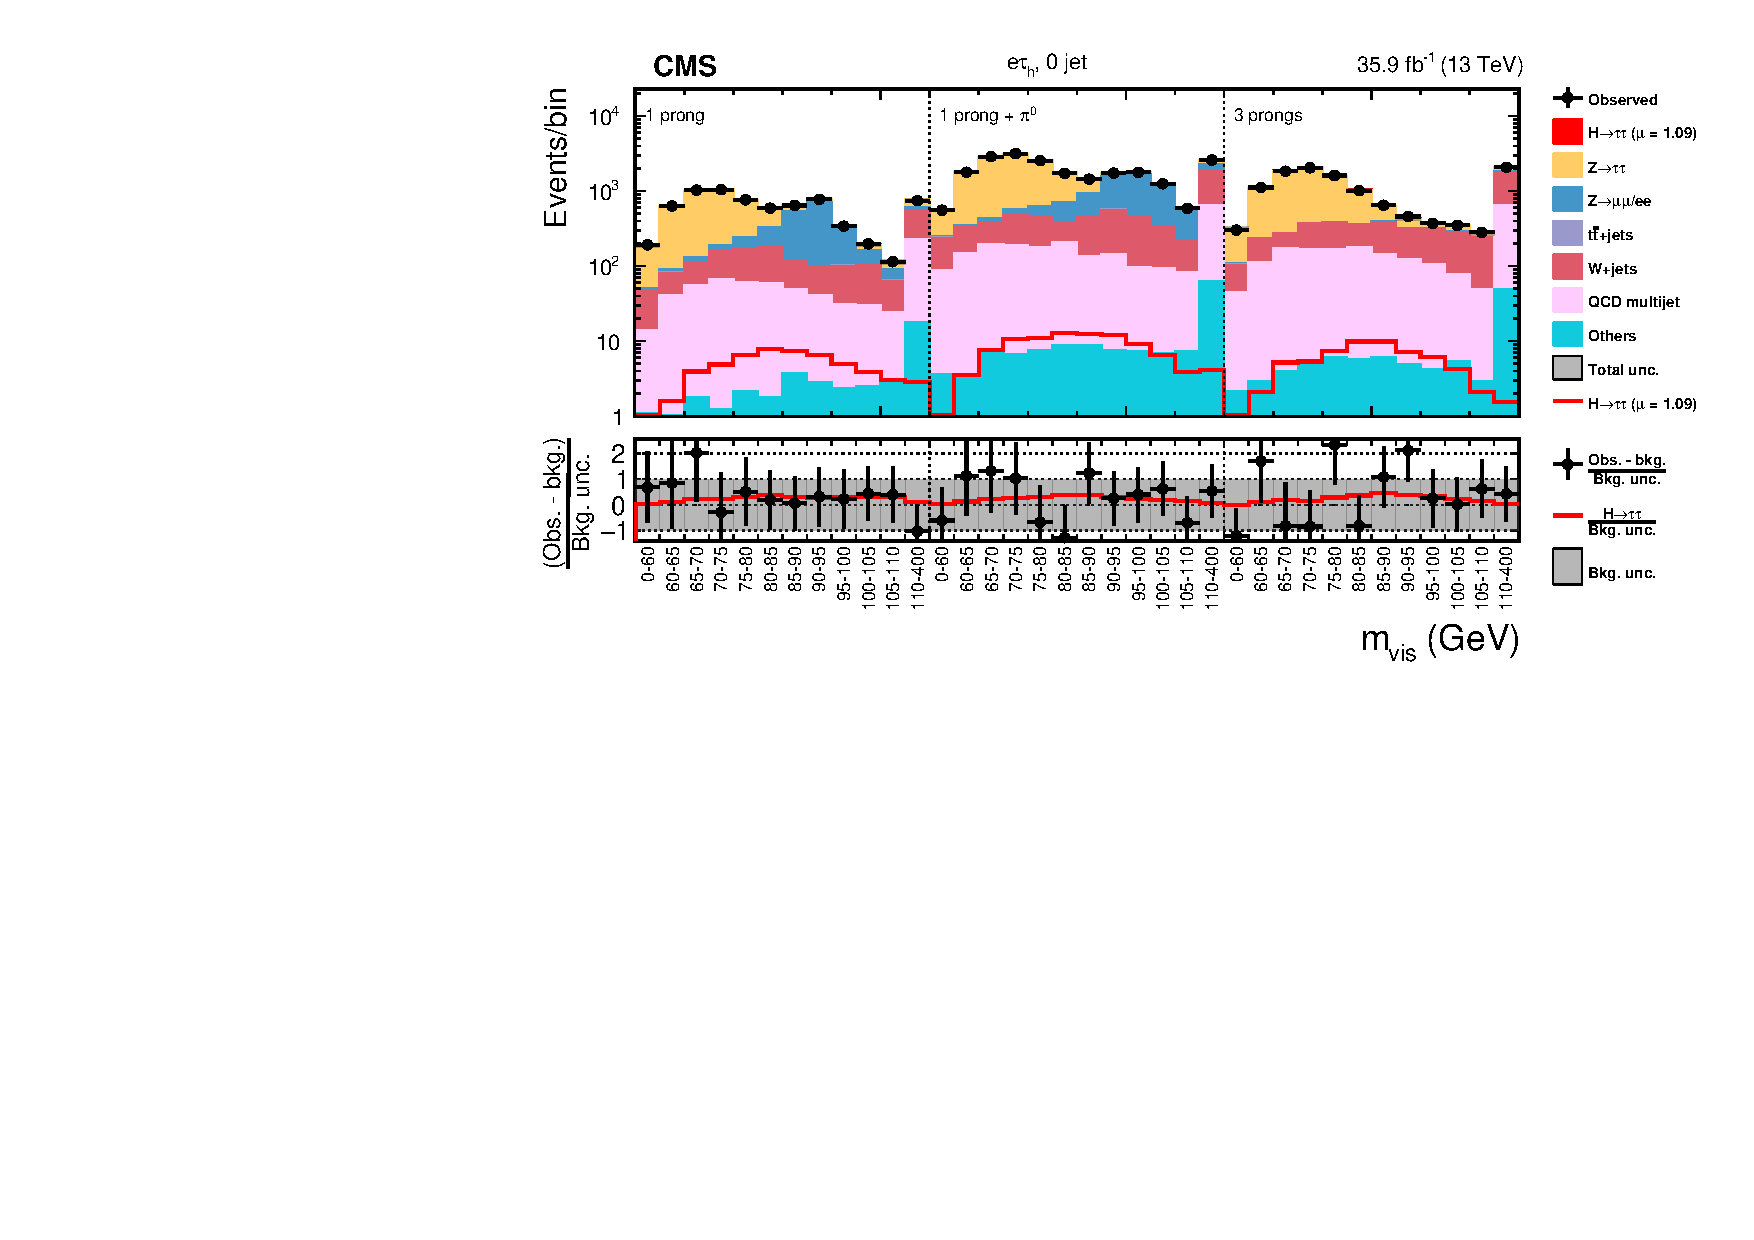
\includegraphics[width=1.0\textwidth]{higgs_to_taus/plots/Figure_016.pdf}
%     \caption{Observed and predicted 2D distributions in the 0-jet category of the $\Pe\tauh$ channel. The description of the histograms is the same as in figure~\ref{fig:mass_tt_vbf}.}
%     \label{fig:mass_et_0jet}
%\end{figure*}
%
%\begin{figure*}[htbp]
%\centering
%     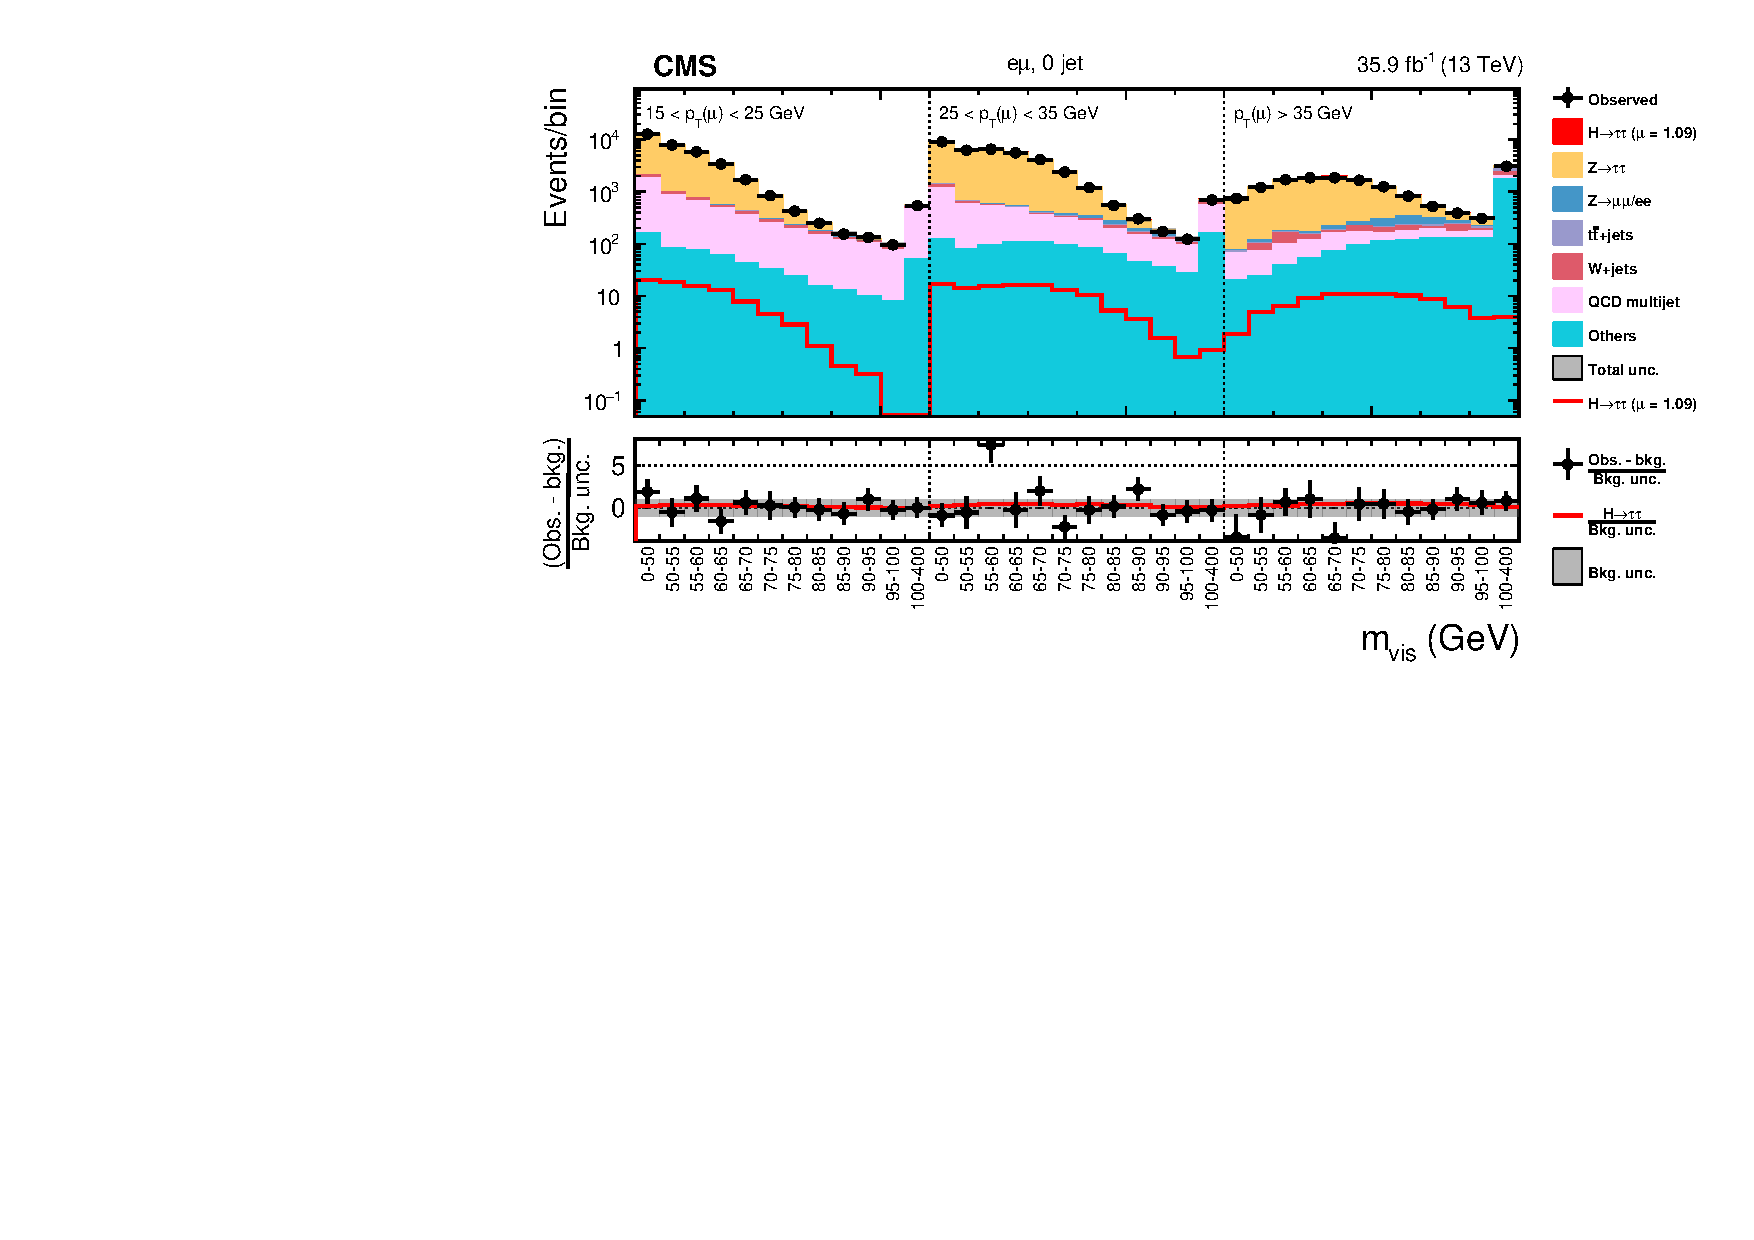
\includegraphics[width=1.0\textwidth]{higgs_to_taus/plots/Figure_017.pdf}
%     \caption{Observed and predicted 2D distributions in the 0-jet category of the $\Pe\Pgm$ channel. The description of the histograms is the same as in figure~\ref{fig:mass_tt_vbf}.}
%     \label{fig:mass_em_0jet}
%\end{figure*}


\section{Results Extraction}
\label{sec:htt_fit_details}
The 2D distributions of the final discriminating variables obtained for each category and each channel in the 
signal regions, along with the control regions, are combined in a binned likelihood fit involving the 
background and signal expectations and observed data in each bin.
The expected number of signal events is the one predicted for the production of
a SM Higgs Boson of mass $\mH=125.09\GeV$ decaying into a pair of $\Pgt$ leptons. In the fit
the number of signal events is
multiplied by a signal strength modifier $\mu$ treated as a free parameter in the fit.

The systematic uncertainties are represented by nuisance parameters that are varied in the fit 
according to their defined probability density functions.
A log-normal probability density function is assumed for the nuisance parameters affecting the event yields 
of the various background contributions such as theory-based cross section uncertainties and
electron, muon, and $\tauh$ reconstruction efficiencies. Systematic uncertainties that affect the shape of the 
distributions, such as the visible $\tauh$ energy scale and \etvecmiss energy scales, are represented 
by nuisance parameters whose variation 
%results in a continuous perturbation of 
%the spectrum~\cite{Conway-PhyStat} and which are 
is assumed to have a Gaussian probability density function.
Overall, the statistical uncertainty in the observed event yields is the dominant source of uncertainty 
for the combined results.


\section{Analysis Sensitivity Details}
The 2D distributions shown in figures~\ref{fig:mass_tt_vbf}--\ref{fig:mass_mt_0jet} give an intuitive
impression of which bins are the most sensitive to the Higgs Boson signal. Each bin in these distributions
can be reordered and group based on the sensitivity of that bin. For visualization purposes only, we regroup 
events in the signal region by their decimal logarithm of the ratio of the signal ($S$) to 
signal-plus-background ($S+B$) in each bin, figure~\ref{fig:htt_sb}. This visualization method helps smooth out statistical
fluctuation visible in the 2D distributions. An excess of observed events with respect to the 
SM background expectation is clearly visible in the most sensitive bins of the analysis.
The details of the expected background and signal contributions and their uncertainties in the most sensitive bins in 
this plot are broken down in table~\ref{tab:htt_sb}. 
These values are compared against the observed number of events in these sensitive bins. 
The table is defined for bins with $\log_{10}(S/(S+B))>-0.9$. The channel that contributes the 
most to these highly sensitive bins is $\tauh\tauh$.

\begin{figure}[htb]
  \centering
    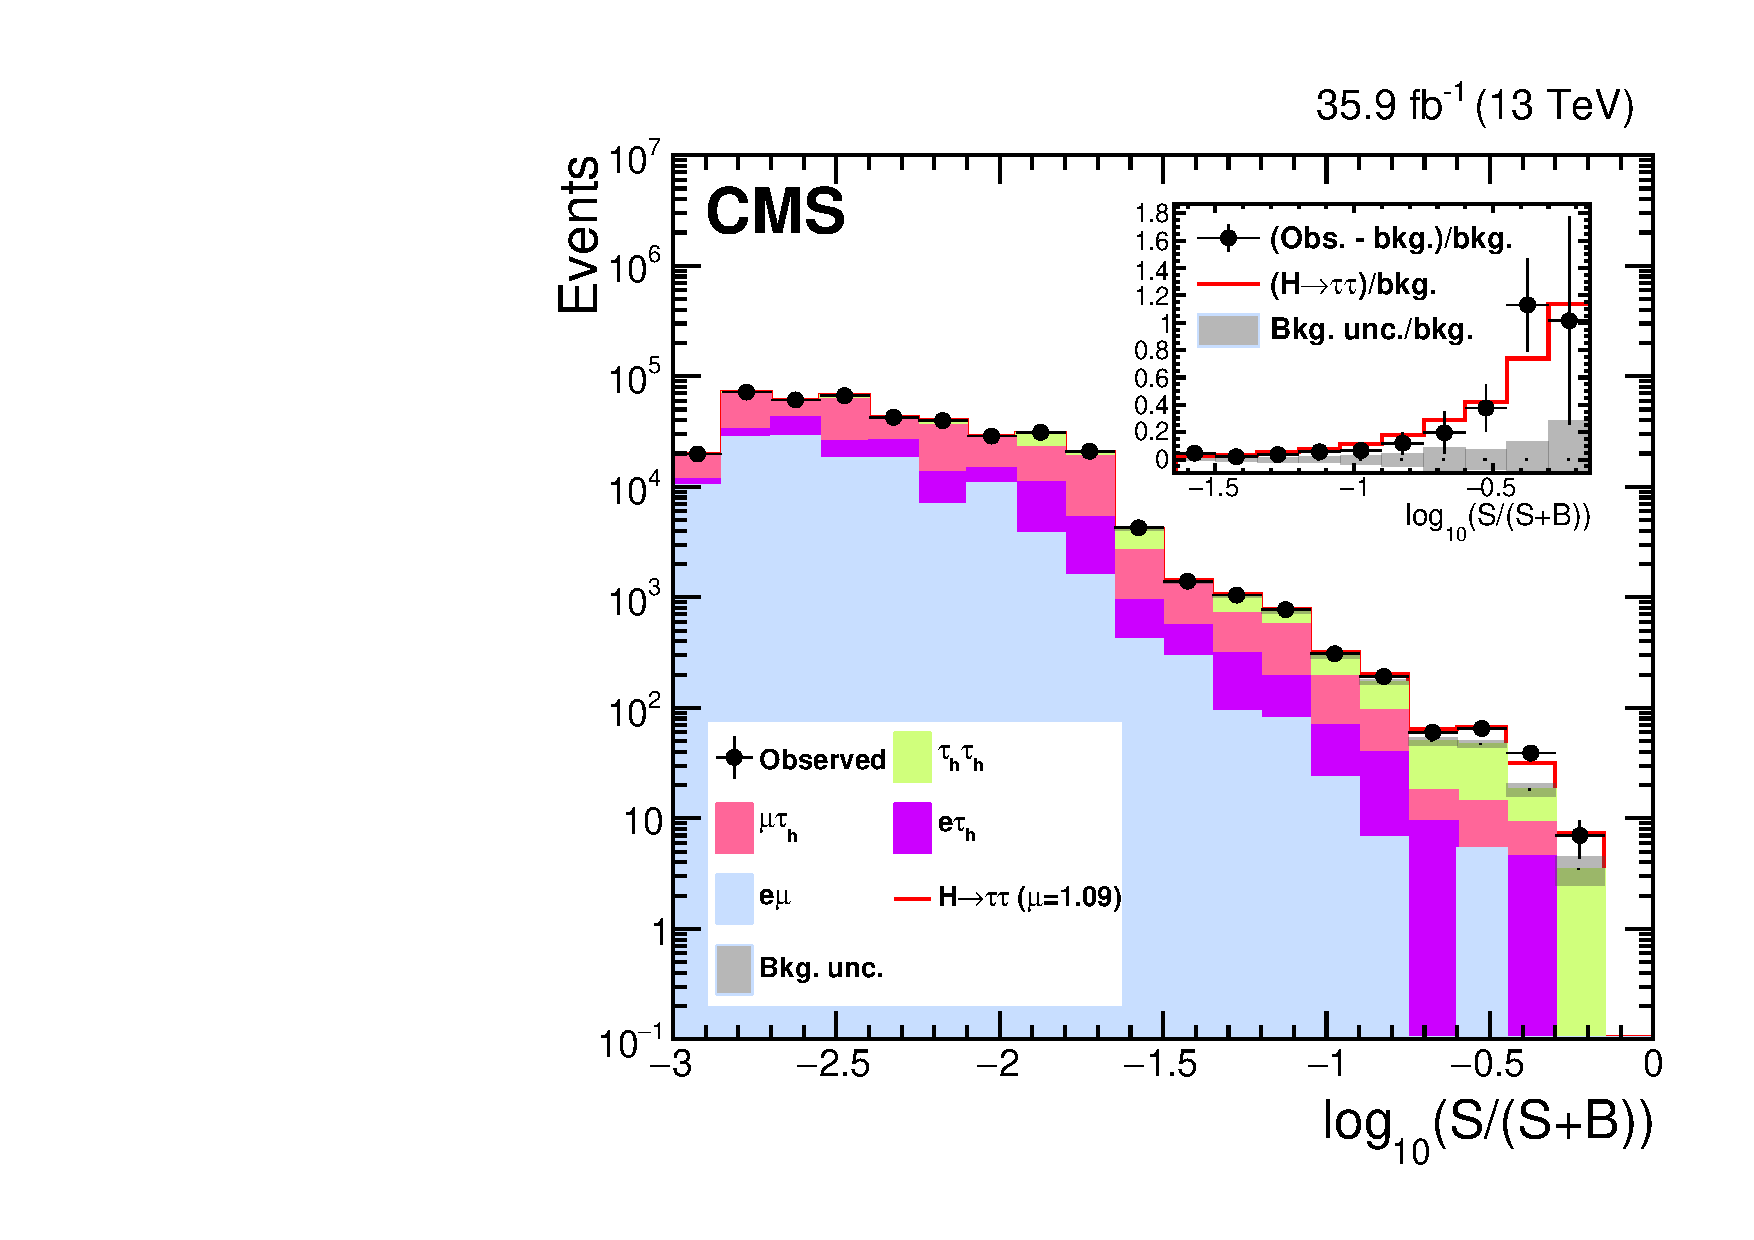
\includegraphics[width=0.65\textwidth]{higgs_to_taus/plots/Figure_018.pdf}
   \caption{Distribution of the decimal logarithm of the ratio between the best fit signal and the sum of 
the best fit signal and best fit background expectations in each bin of the mass distributions used to extract the results.
All signal regions and channels are included. Background contributions are broken down by channel. 
The inset shows the corresponding difference between the observed data and best fit background 
distributions divided by the best fit background expectation. The best fit signal expectation 
is also divided by the background expectation in the inset.
   }
\label{fig:htt_sb}

\end{figure}

\begin{table*}
\centering
\label{tab:htt_sb}
\newcolumntype{x}{D{,}{\,\pm\,}{4.2}}
\begin{tabular}{lxxxx}
Process & \multicolumn{1}{c}{$\Pe\Pgm$} &  \multicolumn{1}{c}{$\Pe\tauh$} &  \multicolumn{1}{c}{$\Pgm\tauh$} &  \multicolumn{1}{c}{$\tauh\tauh$} \\
\hline
$\PZ \to\Pgt\Pgt$ & 5.8, 2.2 & 21.2, 3.3 &34.6, 4.9 & 89.1, 6.9 \\
$\PZ \to \Pe\Pe/\Pgm\Pgm$ & 0.0, 0.0 & 2.9, 0.2 &3.7, 0.2 & 5.0, 0.2 \\
$\ttbar$+jets & 1.9, 0.1 & 10.4, 0.3 &22.2, 1.8 & 13.9, 0.5 \\
$\PW+\text{jets}$ & 0.8, 0.02 & 4.0, 0.3 &6.6, 1.3 & 7.6, 0.8 \\
QCD multijet & 2.1, 0.3 & 3.3, 2.5 &5.0, 1.3 & 35.5, 2.1 \\
Other backgrounds & 1.4, 0.1 & 5.2, 0.2 &6.1, 0.2 & 7.3, 0.2 \\[\cmsTabSkip]
$\Pgg\Pgg\PH, \PH \to\Pgt\Pgt$ & 0.6, 0.1 & 5.0, 0.6 &6.0, 0.6 & 27.4, 2.1  \\
VBF $\PH \to\Pgt\Pgt$ & 2.8, 0.3 & 5.1, 0.5 &12.55, 1.0 & 17.5, 1.0 \\
V$\PH, \PH \to\Pgt\Pgt$ & 0.0, 0.0 & 0.3, 0.0 &0.2, 0.0 & 1.3, 0.1  \\[\cmsTabSkip]
Total backgrounds & 12.1, 2.2 & 46.5, 4.1 &77.7, 5.5 & 156.2, 7.3 \\
Total signal & 3.4, 0.4 & 10.9, 0.8 &19.2, 1.4 & 48.3, 2.6  \\
Observed &  \multicolumn{1}{c}{11} &  \multicolumn{1}{c}{54} &  \multicolumn{1}{c}{91} &  \multicolumn{1}{c}{207}  \\
\hline
\end{tabular}
\caption{Best-fit background and signal expectations, together with the number of observed events, 
for highly sensitive bins in the signal region. High sensitivity bins are defined by $\log_{10}(S/(S+B))>-0.9$, 
where $S$ and $B$ are the number of best fit expected signal events for a Higgs Boson with a mass 
$\mH = 125.09$\GeV and of best fit expected background events. The background uncertainty accounts 
for all sources of background uncertainty, systematic as well as statistical, after the global fit. The 
contribution from ``other backgrounds'' includes events from diboson and single top quark production. 
The contribution from Higgs Boson decays to a pair of $\PW$ bosons is zero in these bins.}
\end{table*}


\section{Mass Distributions}
Another way to visualize the results of the global maximum likelihood fit
is to collapse the second dimension of the 2D distributions. An excess of observed events relative 
to the best fit background expectation is visible in figure~\ref{fig:htt_massweighted},
with the details of the figures construction following.
All of the $\mtt$ distributions with a commong binning scheme are collapsed into a single $\mtt$ distribution.
A reweighting scheme defines a weight for each $\mtt$ range within a slice of $\mjj$ or $\pth$. The reweighting
scheme is designed to increase the contribution of the most sensitive distributions. The reweighting is defined
by summing the best fit background expectations and summing the best fit signal contributions for a given slice
of $\mjj$ or $\pth$; a weight of $S/(S+B)$ is applied to the these contributions when plotting them in the described
distribtion. As a detail $S$ and $B$ are computed as the signal or background contribution in the mass distribution 
excluding the first and last bins, in which the amount of signal is negligible. 
The signal regions that use $\mvis$ instead 
of $\mtt$, namely the 0-jet category of the $\Pgm\tauh$, $\Pe\tauh$ and $\Pe\Pgm$ channels, are not included. 
The different $\mtt$ binning schemes necessitate in two versions of these distributions because the bins
can not be merged a posteriori.
The two different reweighted $\mtt$ distributions are in figure~\ref{fig:htt_massweighted} and group the compatible 
$\mtt$ bins from figures~\ref{fig:mass_tt_vbf}--\ref{fig:mass_mt_0jet}.

\begin{figure}[htb]
  \centering
    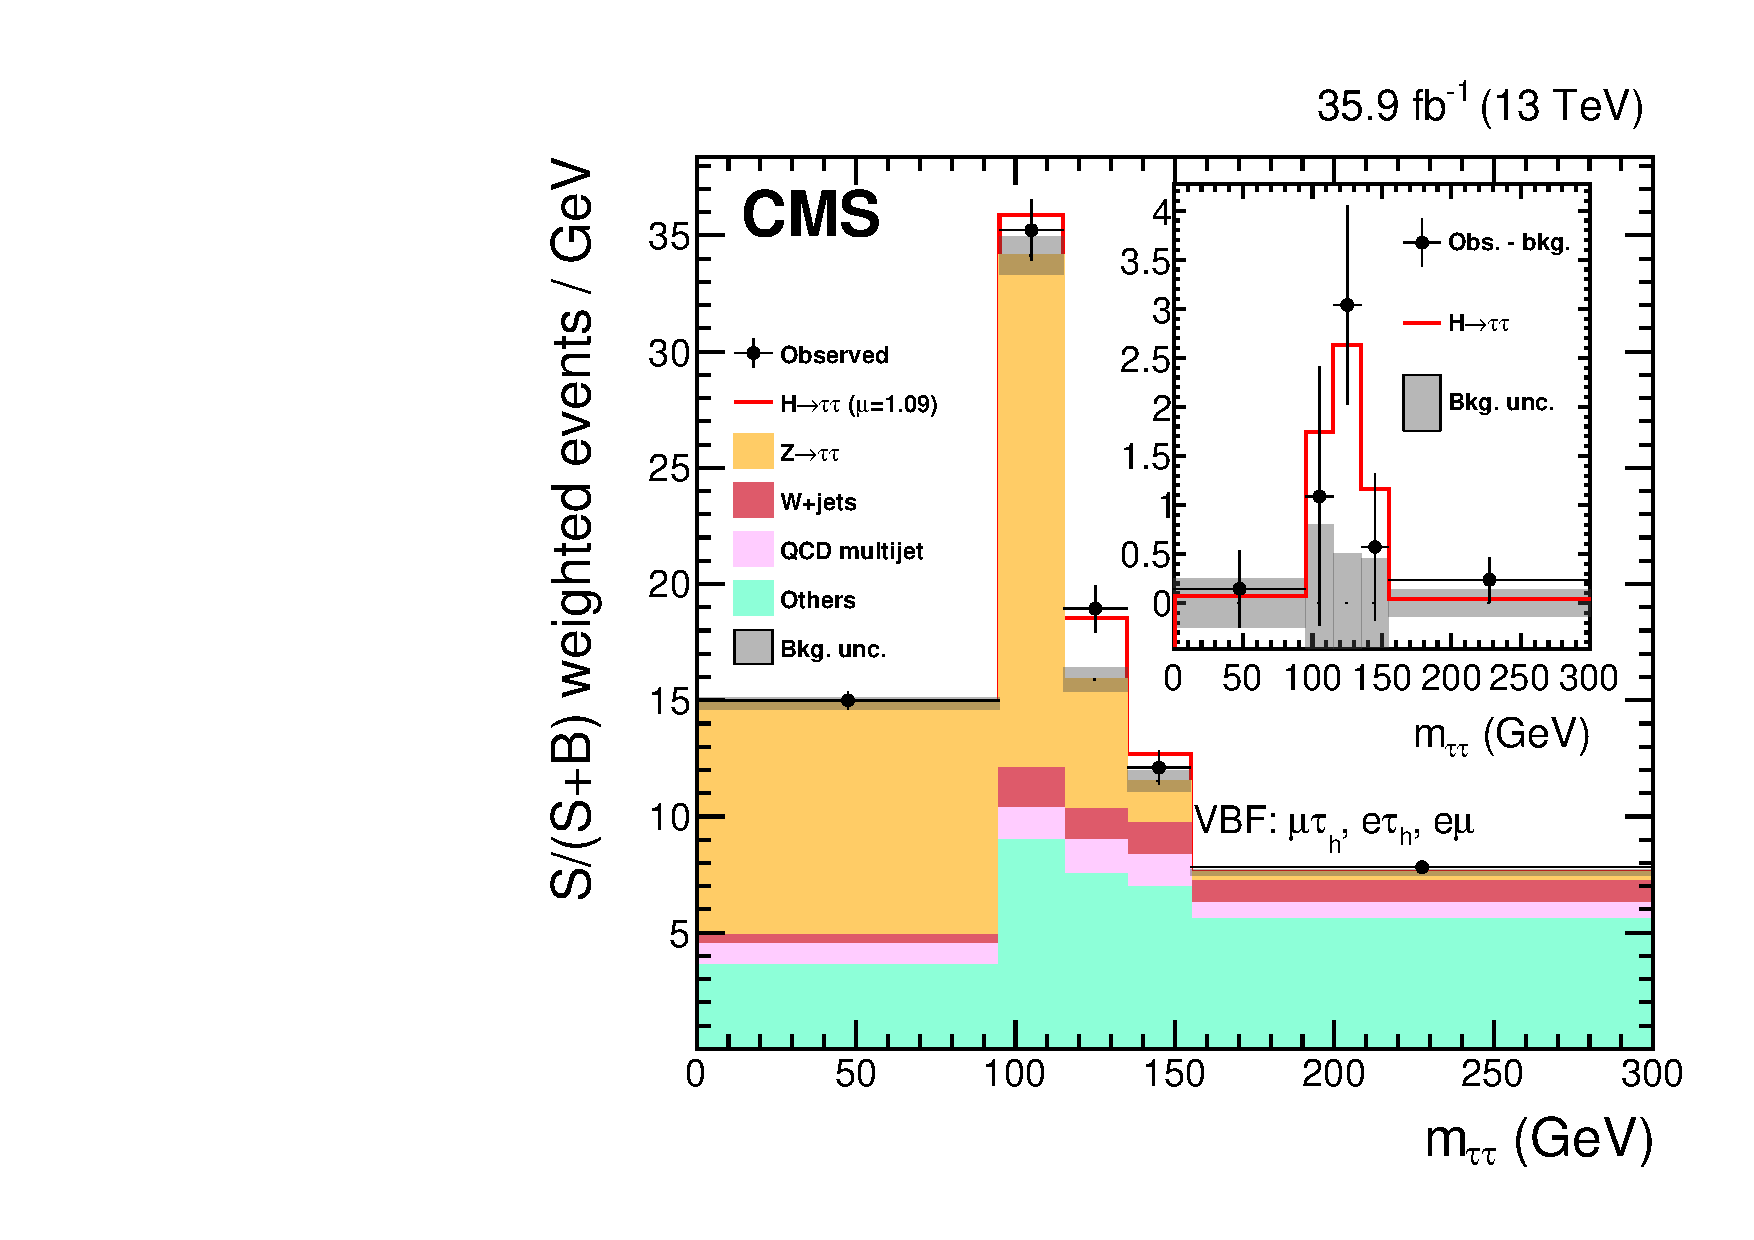
\includegraphics[width=0.48\textwidth]{higgs_to_taus/plots/Figure_019-a.pdf}
    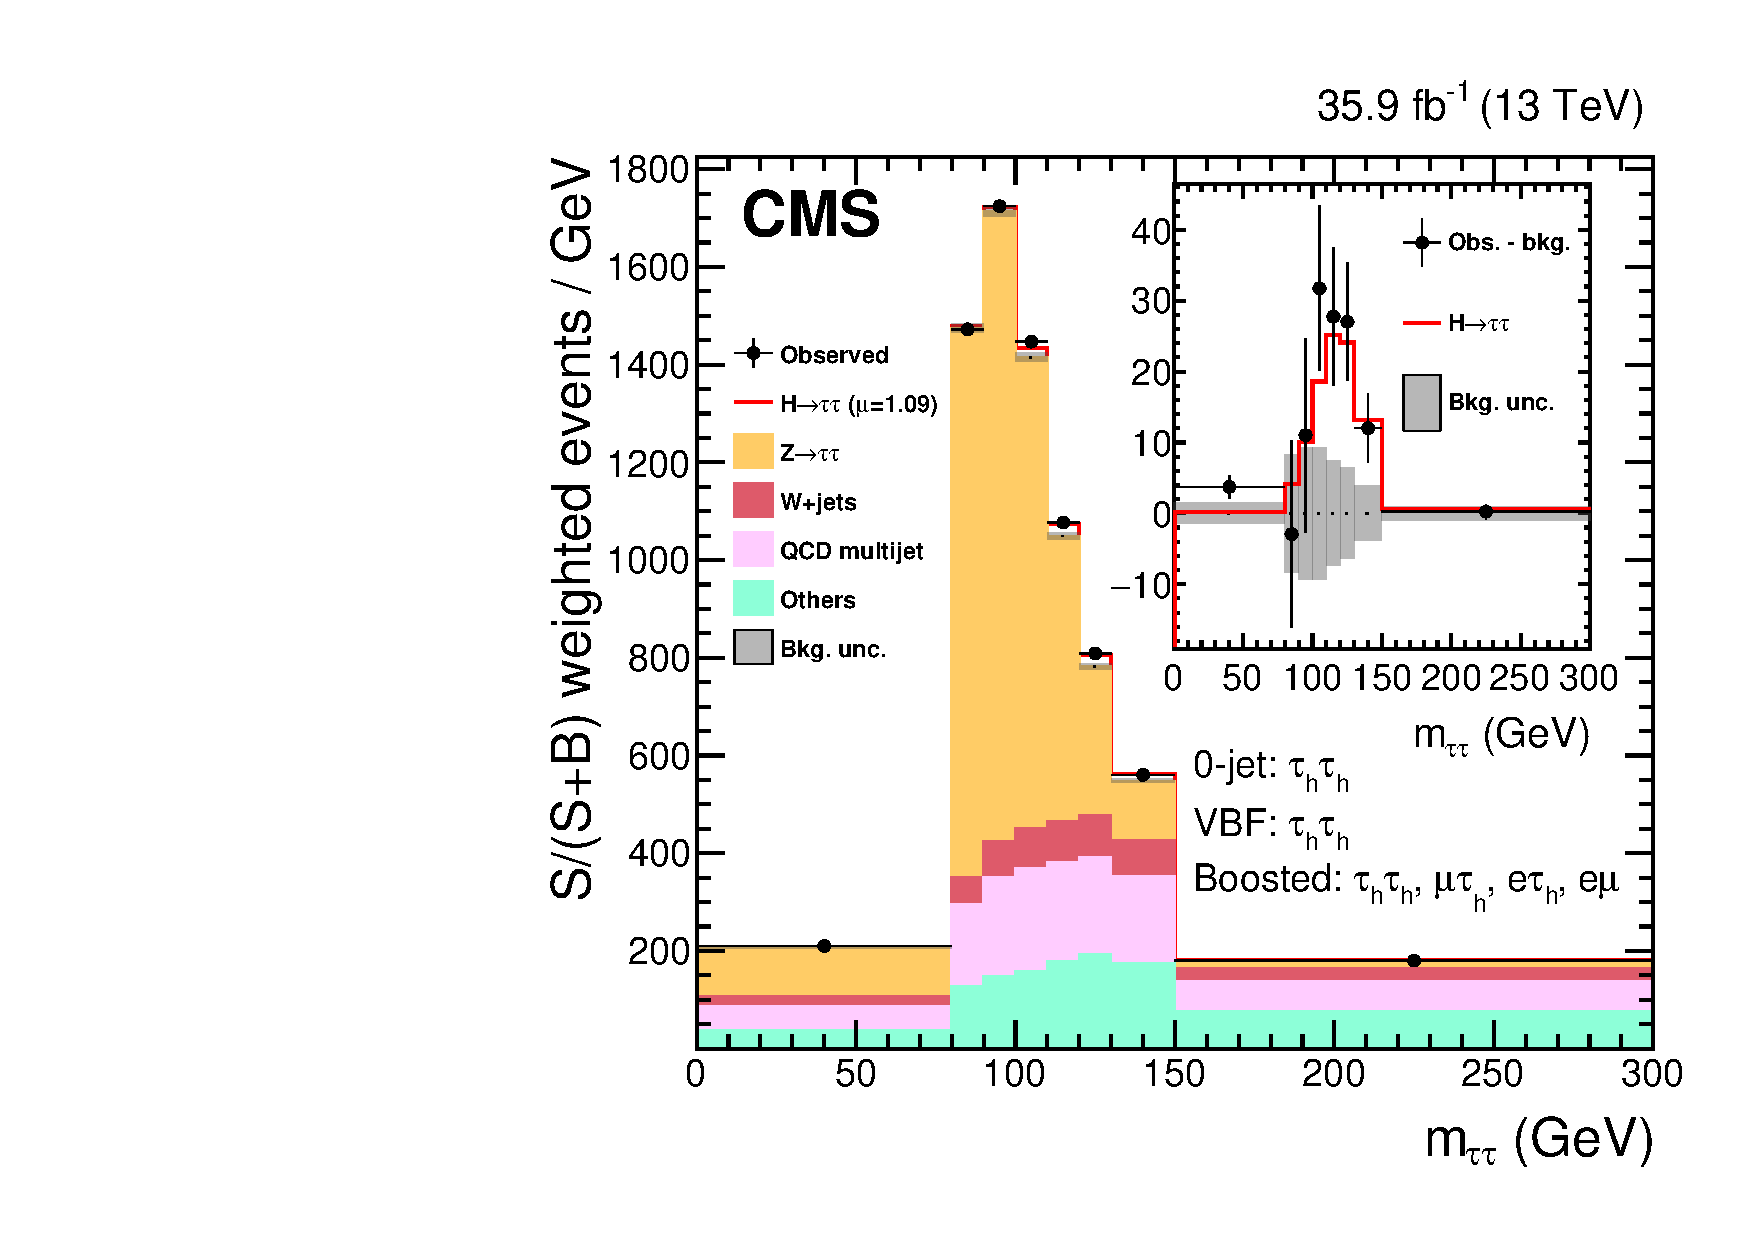
\includegraphics[width=0.48\textwidth]{higgs_to_taus/plots/Figure_019-b.pdf}
   \caption{Combined observed and predicted $\mtt$ distributions. The left pane includes the VBF category of the 
$\Pgm\tauh$, $\Pe\tauh$ and $\Pe\Pgm$ channels, and the right pane includes all other channels that make use 
of $\mtt$ instead of $\mvis$ for the signal strength fit. 
The normalization of the predicted background 
distributions corresponds to the result of the global fit, while the signal is normalized to its best fit 
signal strength. The mass distributions for a constant range of the second dimension of the signal distributions 
are weighted according to $S/(S+B)$, where $S$ and $B$ are computed as the signal or background 
contribution in the mass distributions. The ``Others" background contribution 
includes events from diboson, $\ttbar$, and single top quark production, as well as Higgs Boson decay to a pair 
of $\PW$ bosons and $\PZ$ bosons decaying to a pair of light leptons. The background uncertainty band accounts 
for all sources of background uncertainty, systematic as well as statistical, after the global fit. The inset 
shows the corresponding difference between the observed data and expected background distributions, together 
with the signal expectation. The signal yield is not affected by the reweighting.
}
\label{fig:htt_massweighted}
\end{figure}


\section{Signal Significance And Signal Strength}
The excess in data is quantified by calculating the corresponding local $p$-value using a profile likelihood 
ratio test statistic~\cite{LHC-HCG-Report,Chatrchyan:2012tx,Junk,Read:2002hq} for each Higgs Boson mass
point included in the analysis.
As shown in figure~\ref{fig:htt_pvalue}, the observed significance for a SM Higgs Boson with $\mH = 125.09$\GeV 
is 4.9 standard deviations, for an expected significance of 4.7 standard deviations. Testing multiple mass hypotheses
shows the greatest observed significance for a SM Higgs Boson with the expected SM Higgs Boson value
$\mH = 125.09$\GeV.

\begin{figure}[!ht]
  \centering
    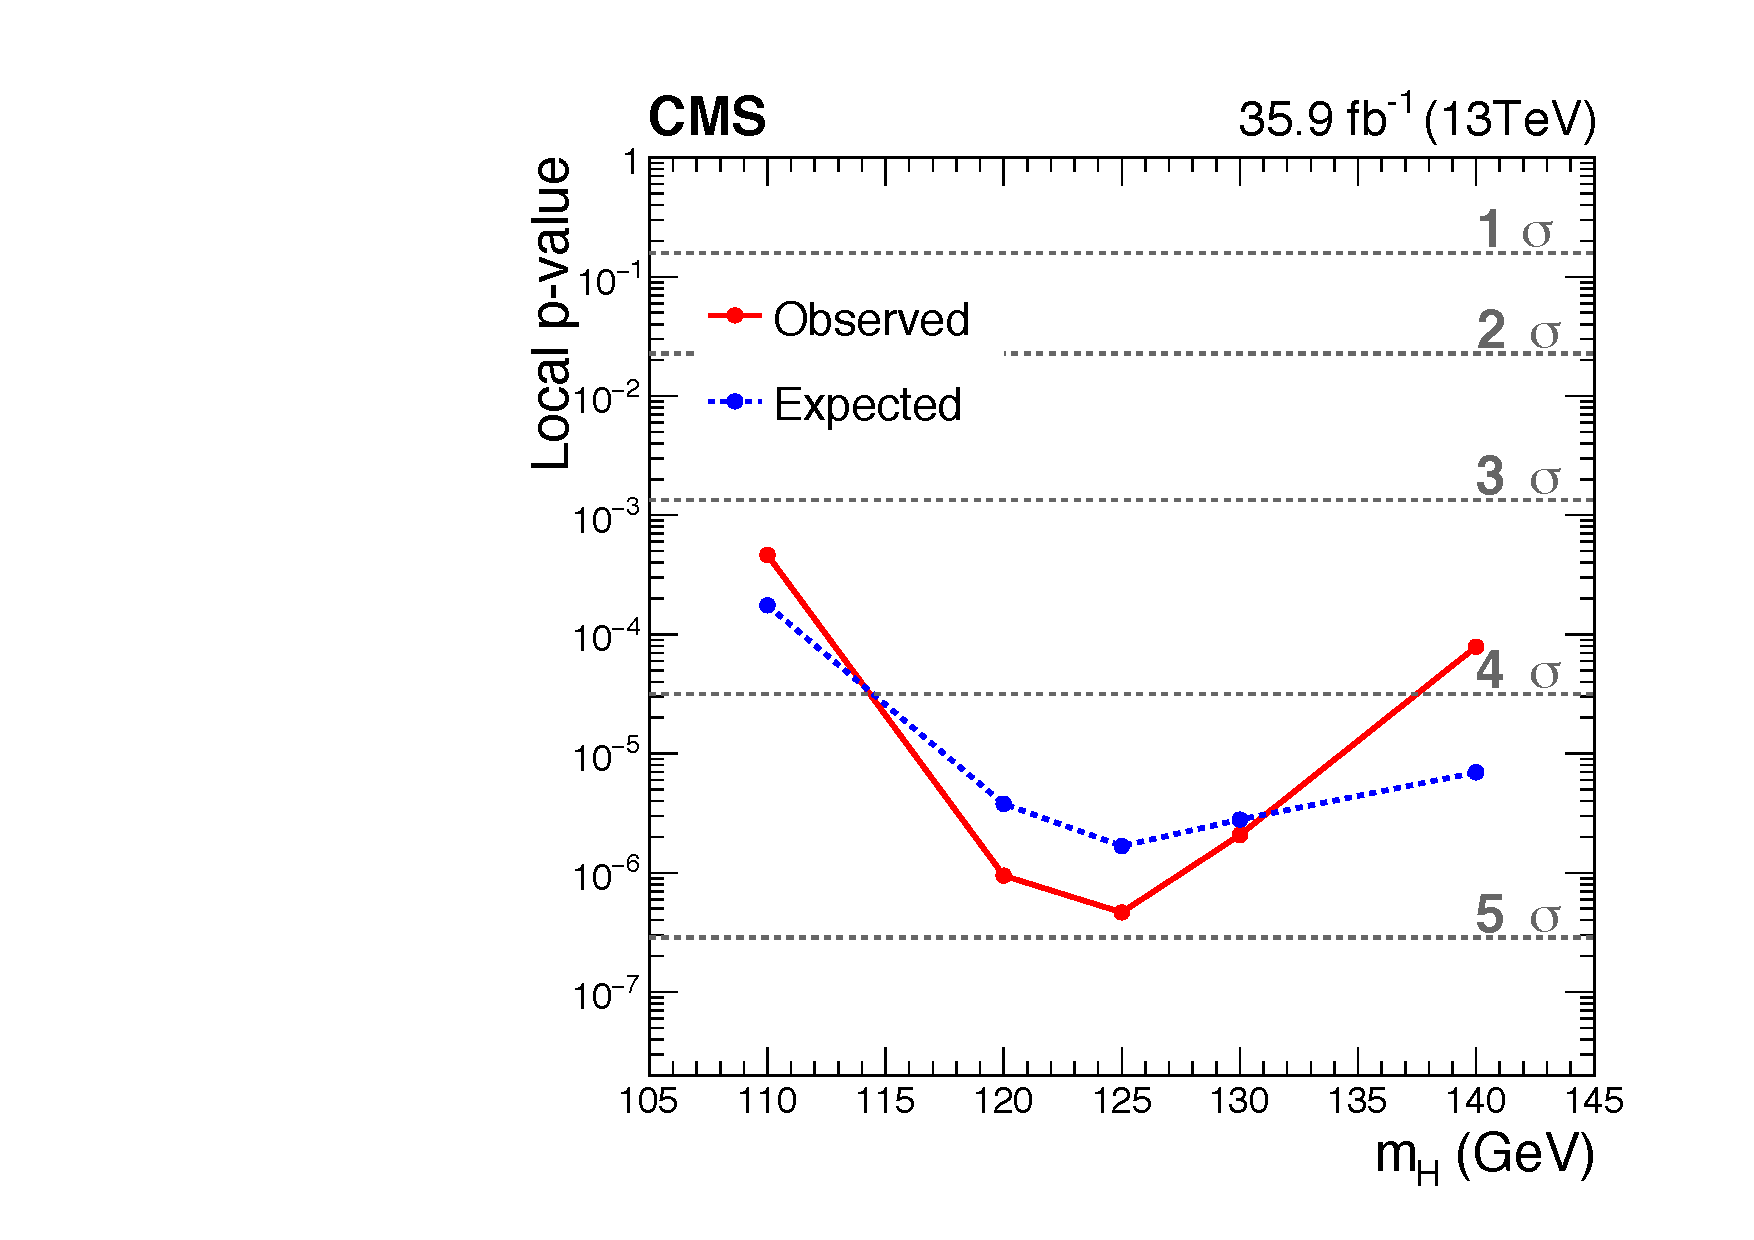
\includegraphics[width=0.5\textwidth]{higgs_to_taus/plots/Figure_020.pdf}
   \caption{Local ${p}$-value and significance as a function of the SM Higgs Boson mass hypothesis. The 
observation (red, solid) is compared to the expectation (blue, dashed) for a Higgs Boson with a mass 
$\mH = 125.09$\GeV. The background includes Higgs Boson decays to pairs of $\PW$ bosons, with $\mH = 125.09$\GeV.}
\label{fig:htt_pvalue}
\end{figure}


The corresponding best fit value for the signal strength $\mu$ is $1.09 ^{+0.27} _{-0.26}$ at $\mH = 125.09\GeV$. 
This result shows very good agreement with the best Standard Model Higgs Boson calculated cross sections
and $\htt$ branching ratio.
The individual best fit signal strengths per channel and per category, using the constraints obtained on the 
systematic uncertainties through the global maximum likelihood fit, are given in figure~\ref{fig:htt_muvalue}; they demonstrate 
the channel- and category-wise consistency of the observation with the SM Higgs Boson hypothesis. The agreement
for each channel and category is within 1 $\sigma$ of the observed signal strength.

\begin{figure}[!ht]
  \centering
    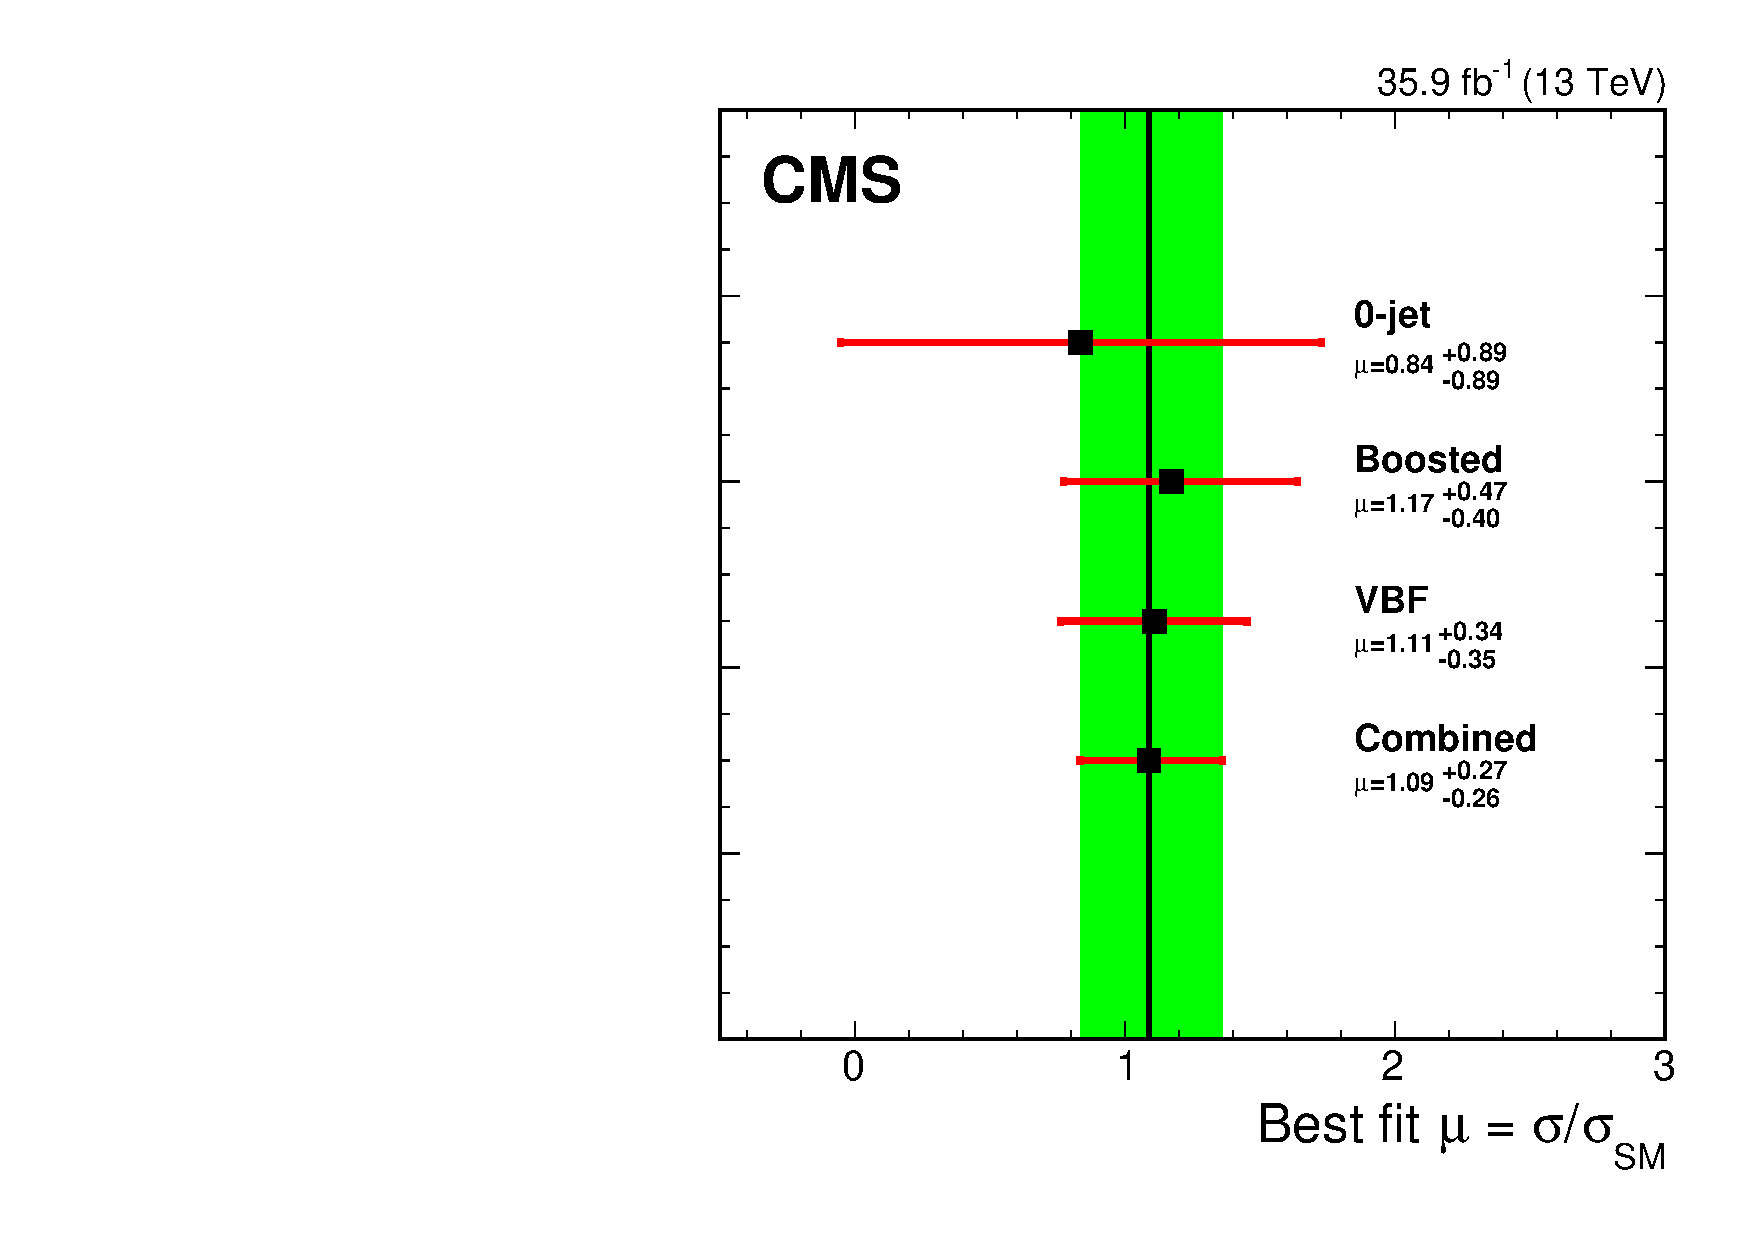
\includegraphics[width=0.49\textwidth]{higgs_to_taus/plots/Figure_021-a.pdf}
    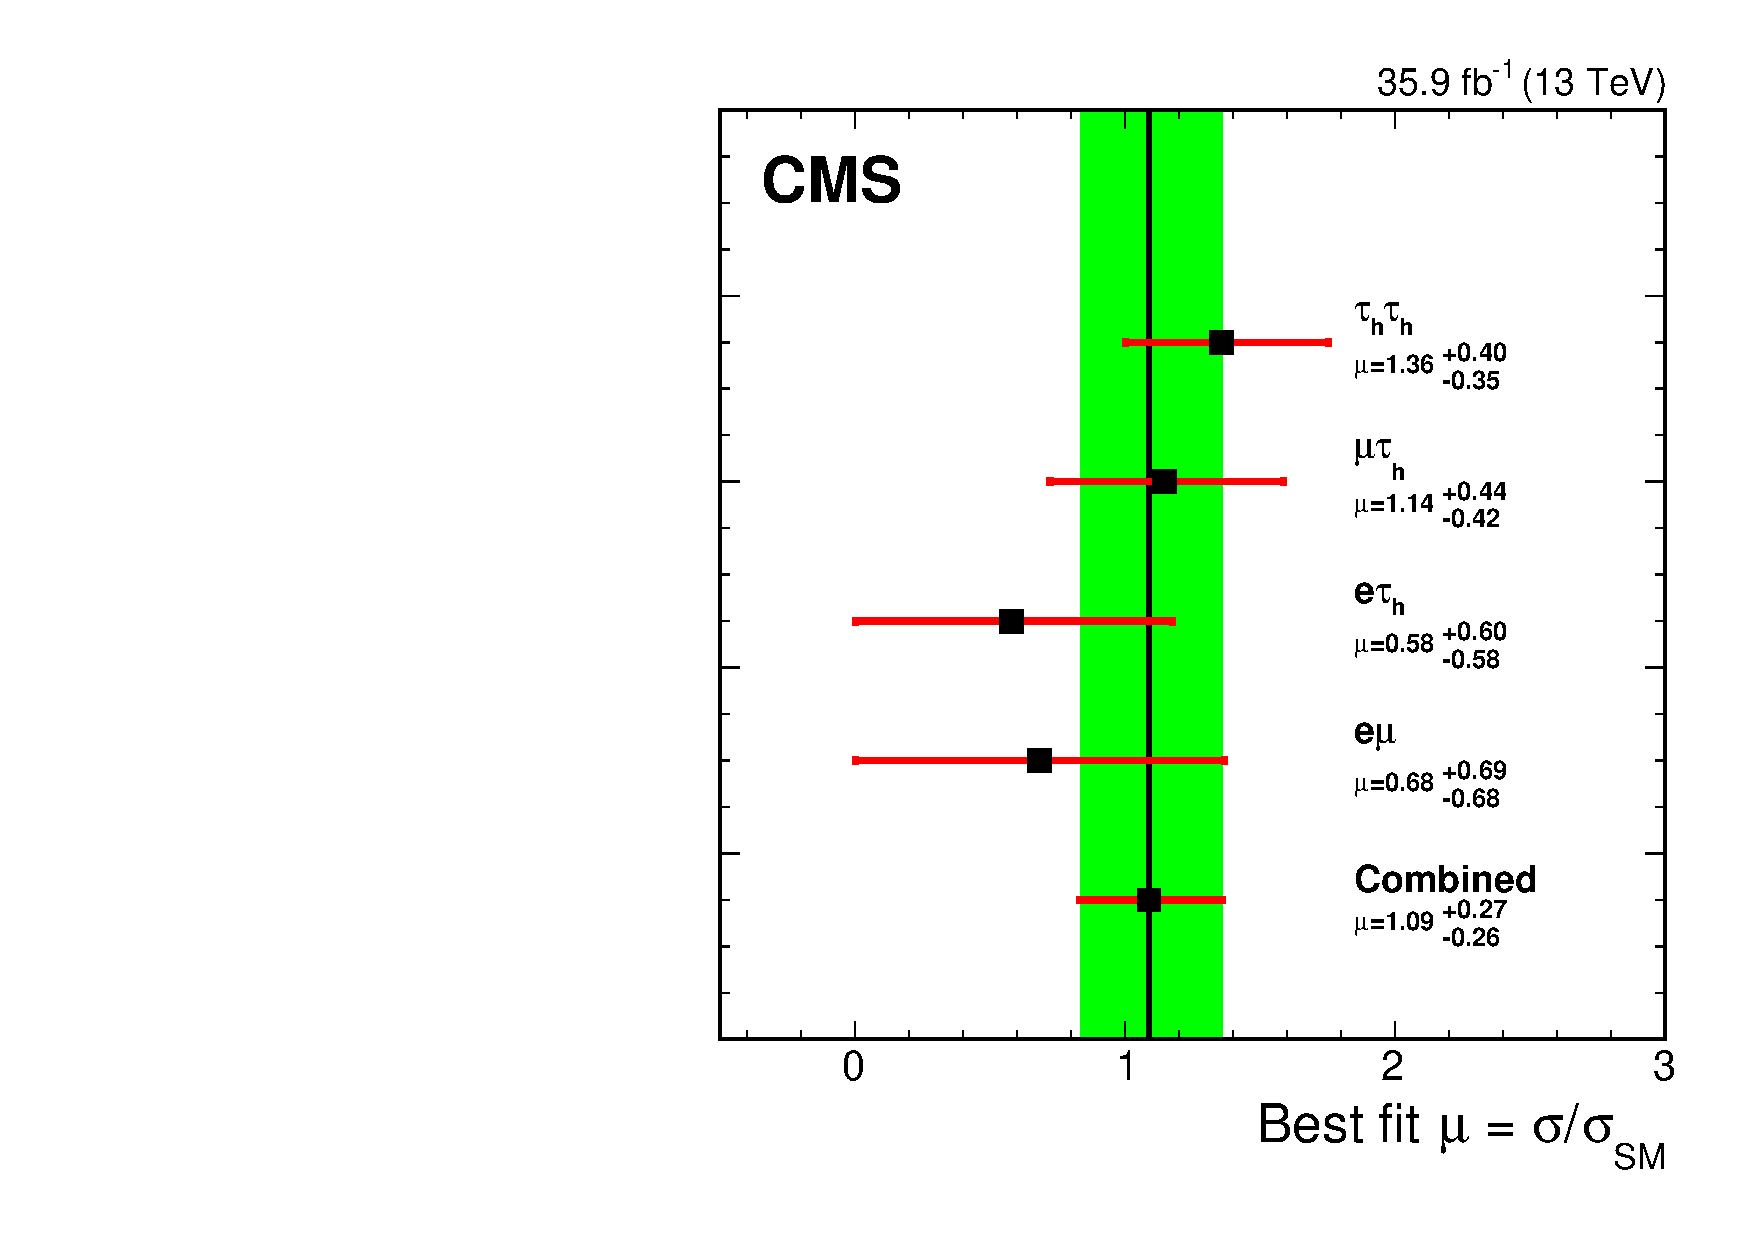
\includegraphics[width=0.49\textwidth]{higgs_to_taus/plots/Figure_021-b.pdf}
   \caption{Best fit signal strength $\mu$ per category (left) and channel (right), for $\mH = 125.09$\GeV. 
The constraints from the global fit are used to extract each of the individual best fit signal strengths. 
The combined best fit signal strength is $\mu = 1.09 ^{+0.27} _{-0.26}$.}
\label{fig:htt_muvalue}
\end{figure}


\section{Higgs Boson Couplings}
\label{sec:htt_kFkV}
A likelihood scan is performed for $\mH=125.09$\GeV in the ($\kappa_\mathrm{V}$,$\kappa_\mathrm{f}$) parameter 
space. $\kappa_\mathrm{V}$ and $\kappa_\mathrm{f}$ quantify the ratio between the measured 
and the SM value for the couplings of the Higgs Boson to vector bosons and fermions, respectively. 
The couplings are considered for both Higgs Boson production and decay.
A full description of the $\kappa$ framework and method used here is described 
in Ref.~\cite{Chatrchyan:2014nva}. For this scan only, Higgs Boson decays to pairs of $\PW$ bosons are 
considered as part of the signal. All nuisance parameters are profiled for each point of the scan. As shown in 
figure~\ref{fig:htt_kVkf}, the observed likelihood contour is consistent with the SM expectation of $\kappa_\mathrm{V}$ 
and $\kappa_\mathrm{f}$ equal to unity.


\begin{figure}[!ht]
  \centering
    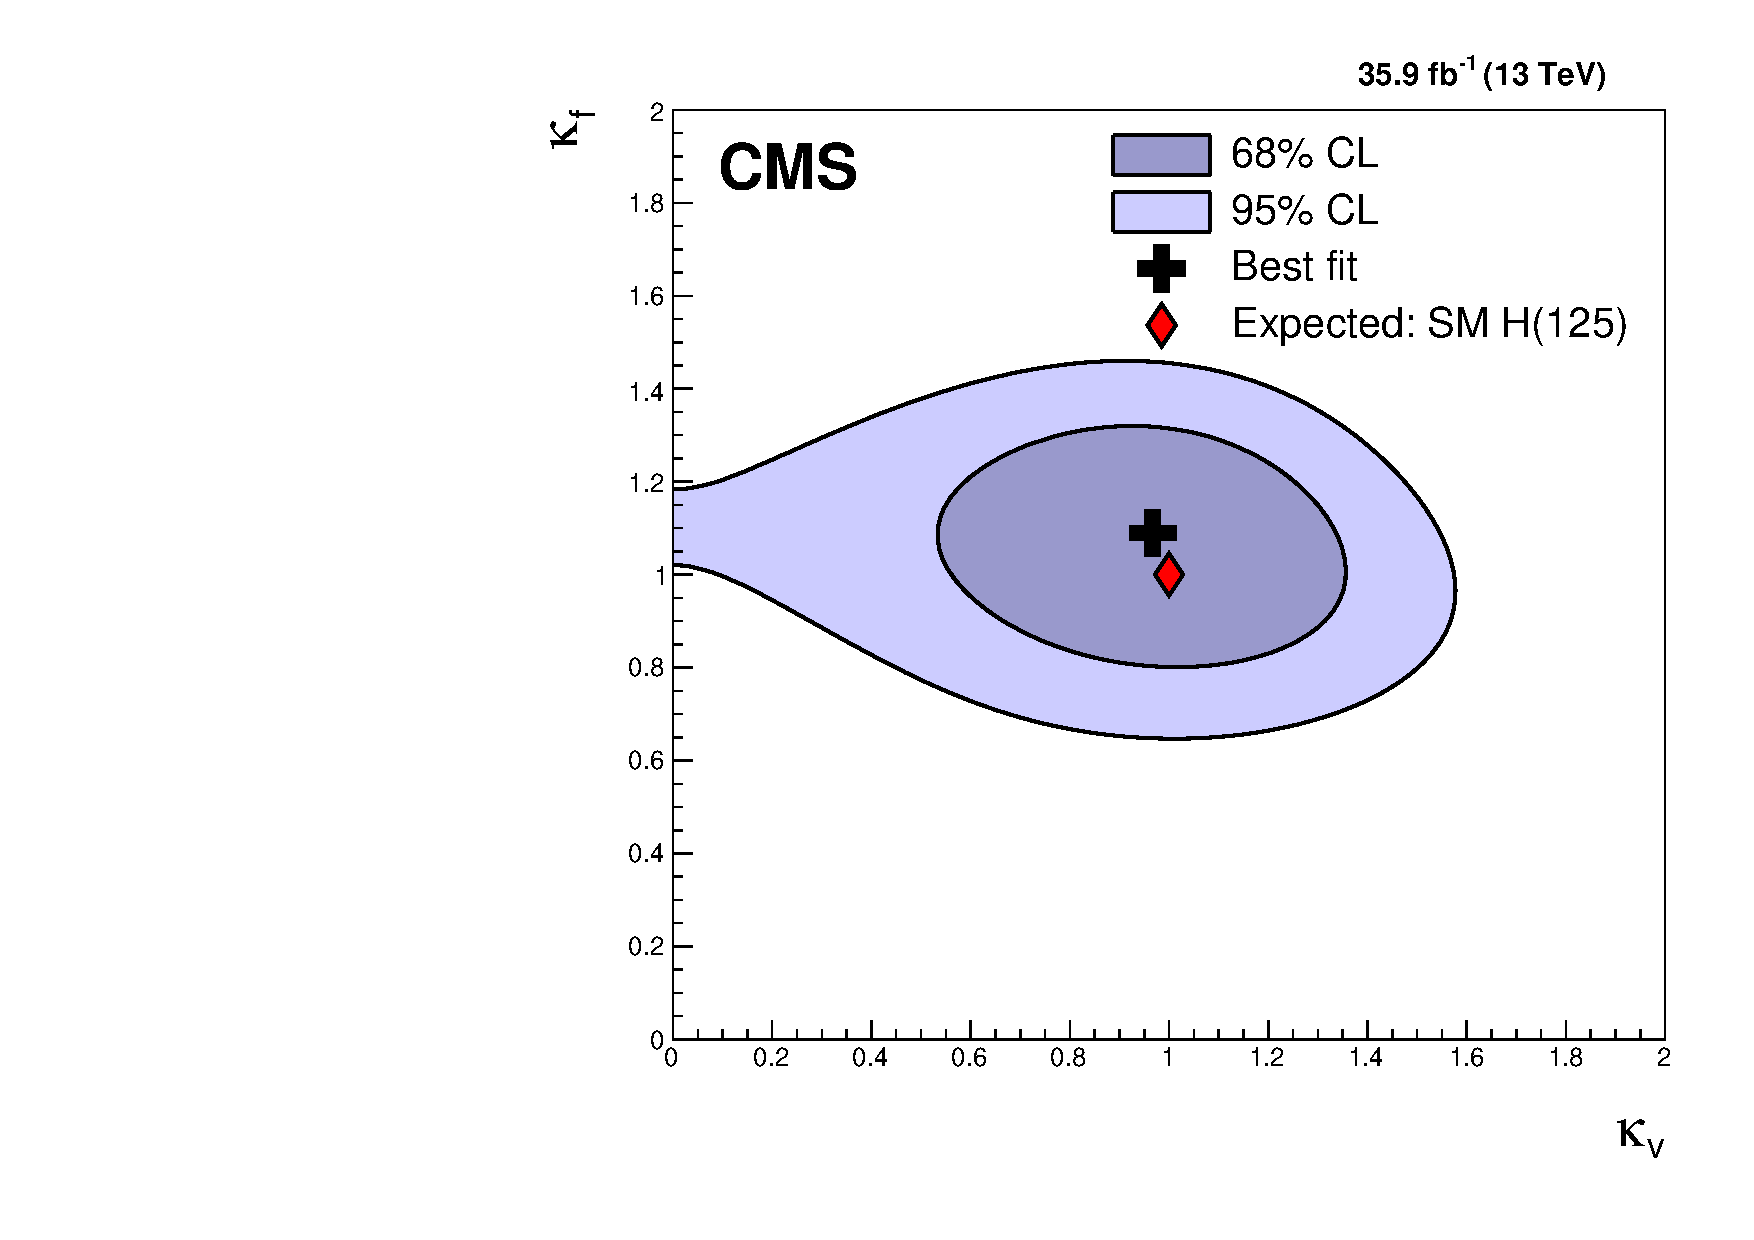
\includegraphics[width=0.65\textwidth]{higgs_to_taus/plots/Figure_022.pdf}
   \caption{Scan of the negative log-likelihood difference as a function of $\kappa_V$ and $\kappa_f$, for 
$\mH = 125.09$\GeV.  All nuisance parameters are profiled for each point. For this scan, the $\Pp\Pp\to \PH\to\PW\PW$ 
contribution is treated as a signal process.}
\label{fig:htt_kVkf}
\end{figure}


\section{Impact of Uncertainties}
The uncertainty on the best fit signal strength, $\mu$, can be decomposed into four components: theoretical uncertainties, 
bin-by-bin statistical uncertainties on the backgrounds, other systematic uncertainties, and the statistical 
uncertainty of the data gathered. In this format, the best fit signal strength is:
\[ \mu = 1.09^{+0.15}_{-0.15}\stat{}^{+0.16}_{-0.15}\syst{}^{+0.10}_{-0.08}\thy{}^{+0.13}_{-0.12} \text{(bin-by-bin).}\]
The impact of these uncertainties on the signal strength was assess by performing a 1D likelihood scan of 
the signal strength with multiple uncertainty hypotheses. These scans can be seen in 
figure~\ref{fig:htt_systematic_parabola}. In different versions of the likelihood scan
certain uncertainty groups were frozen to their best fit values when $\mu = 1.09$. When an uncertainty group is frozen to
its best fit value and not allowed to fluctuate in the likelihood scan, the impact of that uncertainty is
effectively removed from the likelihood calculation process. The resulting likelihood parabola shows how
the results would differ if the frozen uncertainty group did not exist. The difference between the nominal
likelihood parabola and one with frozen uncertainties provides a numerical uncertainty value associated with
the frozen uncertainty group.


\begin{figure*}[htbp]
\centering
     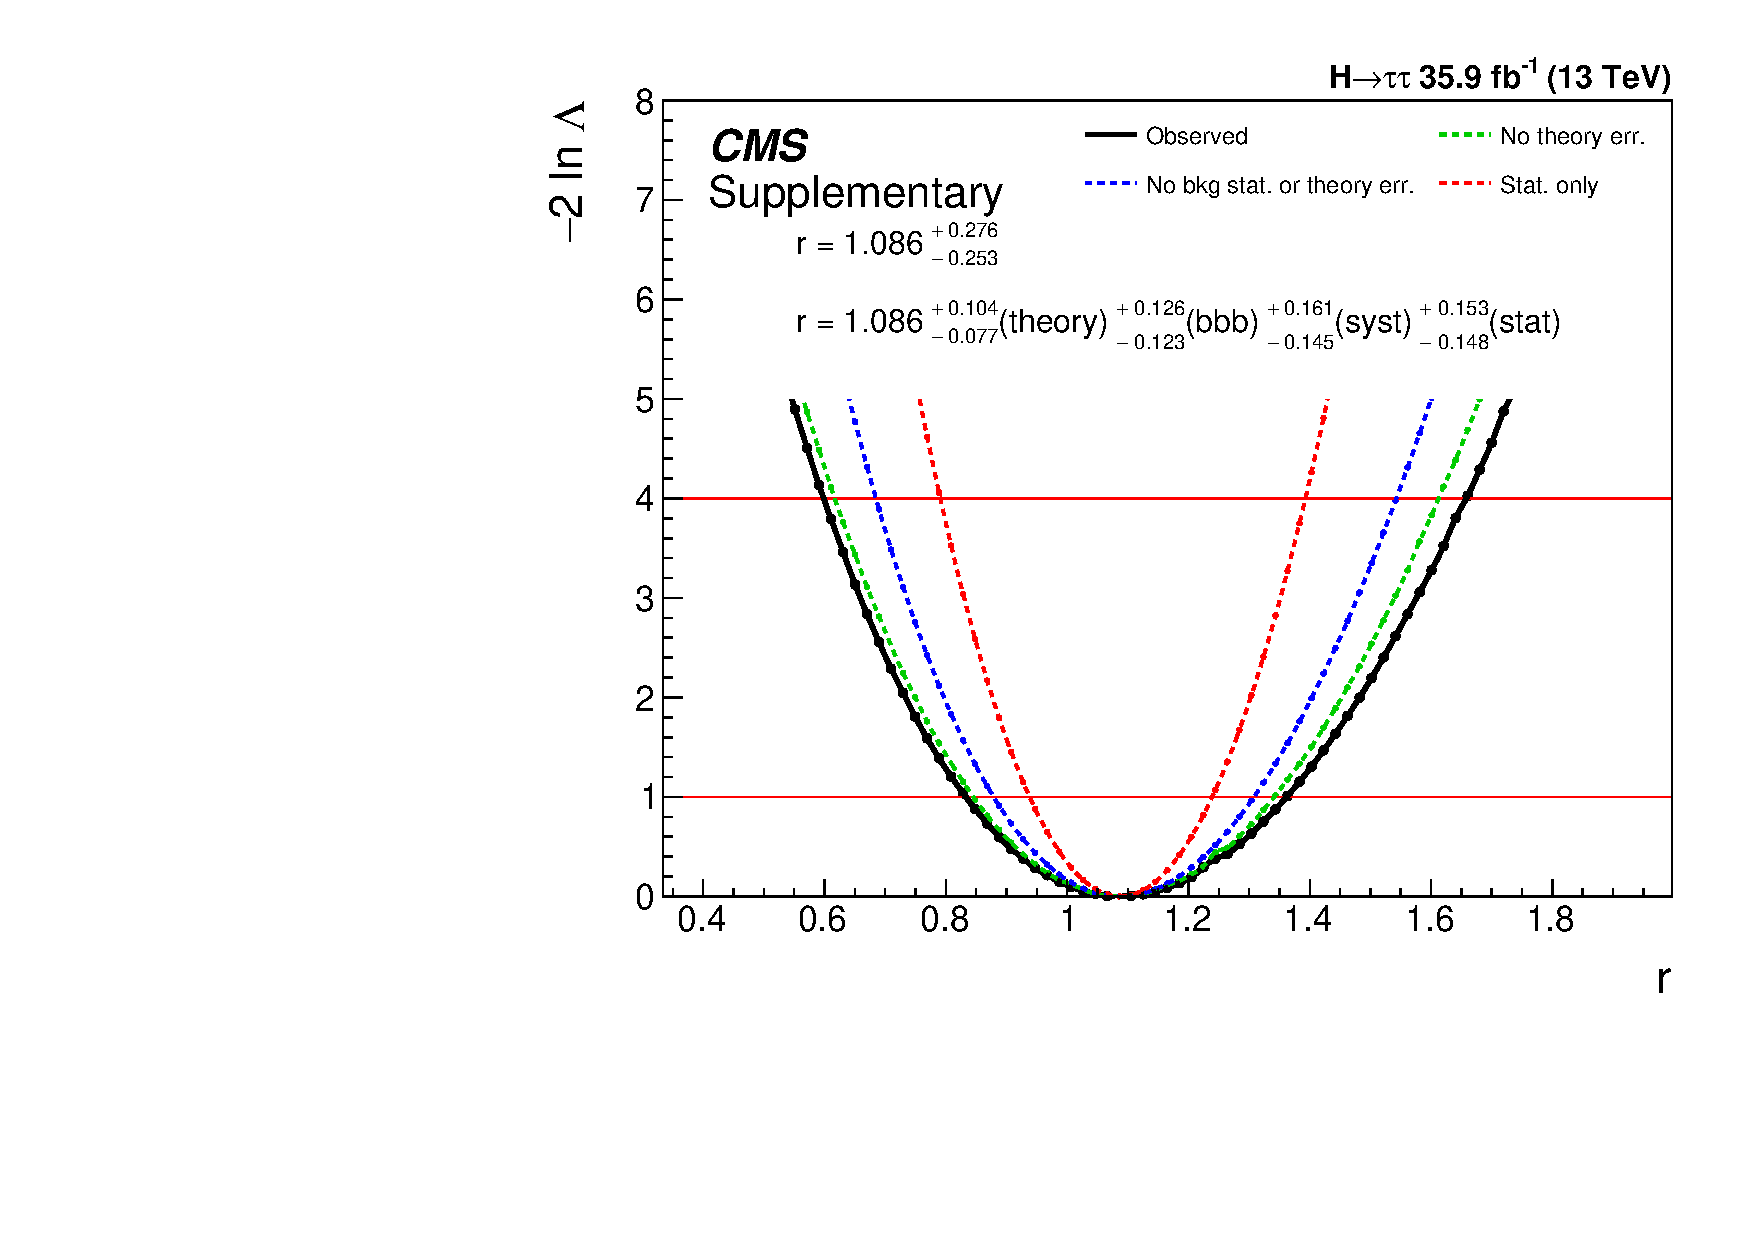
\includegraphics[width=0.70\textwidth]{higgs_to_taus/plots/cms_output_freeze_All_Theory_bbb}\\
     \caption{
1D likelihood scans which were used to extract the uncertainty associated with each of the four uncertainty
components: theoretical uncertainties, bin-by-bin statistical uncertainties on the backgrounds, other 
systematic uncertainties, and the statistical uncertainty of the data gathered. The difference between
the nominal scan in black and the scans representd as dotted lines show the effect of freezing out certain
uncertainty components from the analysis. Freezing out an uncertainty component shows how the analysis
results would change if there was zero uncertainty associated with that component. For example, the green
dotted curve shows how the analysis results would change if theoretical Higgs Boson uncertainties were
reduced to zero.
}
     \label{fig:htt_systematic_parabola}
\end{figure*}


\section{Combination with Run-I Results}
The results of this study are combined with the results of the search for $\PH\to\Pgt\Pgt$ performed with the data collected with 
the CMS detector at center-of-mass energies of 7 and 8\TeV~\cite{Khachatryan:2014jba}. A common signal strength is used
for all data taking periods. All uncertainties are considered as fully uncorrelated between the different 
center-of-mass energies. The combination of these two results leads to an observed and an expected significance of 5.9 standard 
deviations. The corresponding best fit value for the signal strength $\mu$ is $0.98\pm 0.18$ at 
$\mH = 125.09\GeV$. This constitutes the most significant direct measurement of the coupling of the Higgs Boson 
to fermions by a single experiment.

The 13 TeV $\htt$ analysis using data gathered by the CMS experiment in 2016 discussed here provides the first 
single-experiment observation of the SM Higgs Boson decaying to fermions. This is a very important benchmark for the CMS
experiment and the high energy particle physics commuinty as a whole. There is still room to improve this
measurement using the 2016 13 TeV center-of-mass energy data collected by the CMS experiment. The analysis
detailed here did not include any channels dedicated to targeting Higgs Bosons produced in associated production.
The following chapter discusses the $\PW/\PZ+\PH$, with $\htt$ analysis.


